\documentclass[twoside]{book}

% Packages required by doxygen
\usepackage{fixltx2e}
\usepackage{calc}
\usepackage{doxygen}
\usepackage[export]{adjustbox} % also loads graphicx
\usepackage{graphicx}
\usepackage[utf8]{inputenc}
\usepackage{makeidx}
\usepackage{multicol}
\usepackage{multirow}
\PassOptionsToPackage{warn}{textcomp}
\usepackage{textcomp}
\usepackage[nointegrals]{wasysym}
\usepackage[table]{xcolor}

% Font selection
\usepackage[T1]{fontenc}
\usepackage[scaled=.90]{helvet}
\usepackage{courier}
\usepackage{amssymb}
\usepackage{sectsty}
\renewcommand{\familydefault}{\sfdefault}
\allsectionsfont{%
  \fontseries{bc}\selectfont%
  \color{darkgray}%
}
\renewcommand{\DoxyLabelFont}{%
  \fontseries{bc}\selectfont%
  \color{darkgray}%
}
\newcommand{\+}{\discretionary{\mbox{\scriptsize$\hookleftarrow$}}{}{}}

% Page & text layout
\usepackage{geometry}
\geometry{%
  a4paper,%
  top=2.5cm,%
  bottom=2.5cm,%
  left=2.5cm,%
  right=2.5cm%
}
\tolerance=750
\hfuzz=15pt
\hbadness=750
\setlength{\emergencystretch}{15pt}
\setlength{\parindent}{0cm}
\setlength{\parskip}{3ex plus 2ex minus 2ex}
\makeatletter
\renewcommand{\paragraph}{%
  \@startsection{paragraph}{4}{0ex}{-1.0ex}{1.0ex}{%
    \normalfont\normalsize\bfseries\SS@parafont%
  }%
}
\renewcommand{\subparagraph}{%
  \@startsection{subparagraph}{5}{0ex}{-1.0ex}{1.0ex}{%
    \normalfont\normalsize\bfseries\SS@subparafont%
  }%
}
\makeatother

% Headers & footers
\usepackage{fancyhdr}
\pagestyle{fancyplain}
\fancyhead[LE]{\fancyplain{}{\bfseries\thepage}}
\fancyhead[CE]{\fancyplain{}{}}
\fancyhead[RE]{\fancyplain{}{\bfseries\leftmark}}
\fancyhead[LO]{\fancyplain{}{\bfseries\rightmark}}
\fancyhead[CO]{\fancyplain{}{}}
\fancyhead[RO]{\fancyplain{}{\bfseries\thepage}}
\fancyfoot[LE]{\fancyplain{}{}}
\fancyfoot[CE]{\fancyplain{}{}}
\fancyfoot[RE]{\fancyplain{}{\bfseries\scriptsize Generated by Doxygen }}
\fancyfoot[LO]{\fancyplain{}{\bfseries\scriptsize Generated by Doxygen }}
\fancyfoot[CO]{\fancyplain{}{}}
\fancyfoot[RO]{\fancyplain{}{}}
\renewcommand{\footrulewidth}{0.4pt}
\renewcommand{\chaptermark}[1]{%
  \markboth{#1}{}%
}
\renewcommand{\sectionmark}[1]{%
  \markright{\thesection\ #1}%
}

% Indices & bibliography
\usepackage{natbib}
\usepackage[titles]{tocloft}
\setcounter{tocdepth}{3}
\setcounter{secnumdepth}{5}
\makeindex

% Hyperlinks (required, but should be loaded last)
\usepackage{ifpdf}
\ifpdf
  \usepackage[pdftex,pagebackref=true]{hyperref}
\else
  \usepackage[ps2pdf,pagebackref=true]{hyperref}
\fi
\hypersetup{%
  colorlinks=true,%
  linkcolor=blue,%
  citecolor=blue,%
  unicode%
}

% Custom commands
\newcommand{\clearemptydoublepage}{%
  \newpage{\pagestyle{empty}\cleardoublepage}%
}

\usepackage{caption}
\captionsetup{labelsep=space,justification=centering,font={bf},singlelinecheck=off,skip=4pt,position=top}

%===== C O N T E N T S =====

\begin{document}

% Titlepage & ToC
\hypersetup{pageanchor=false,
             bookmarksnumbered=true,
             pdfencoding=unicode
            }
\pagenumbering{alph}
\begin{titlepage}
\vspace*{7cm}
\begin{center}%
{\Large My Project }\\
\vspace*{1cm}
{\large Generated by Doxygen 1.8.13}\\
\end{center}
\end{titlepage}
\clearemptydoublepage
\pagenumbering{roman}
\tableofcontents
\clearemptydoublepage
\pagenumbering{arabic}
\hypersetup{pageanchor=true}

%--- Begin generated contents ---
\chapter{Assignment 1\+: Joseph Seklawy -\/ 12578845}
\label{index}\hypertarget{index}{}The task is to simulates the generation of data from several sensor(rangers) types, and performs data fusion.

Users will have to initiate the sensors they wish to use within the main and then using the varius set functions available in the \hyperlink{ranger_8h_source}{ranger.\+h} class header, they can then set the various parameters they wish to change. These sensors should then be passed into a vector which itself is passed to the \hyperlink{classRangerFusion}{Ranger\+Fusion} class constructor. Once the code is run, the user will be prompted to input the number of cells they wish to create to be checked by the sensors created beforehand. The sensors will then randomly generate data based on the inputed variables and its specifications, and that data will be run through the Graband\+Fuse\+Data function which determines based on the sensor readings whether a cell is free, occupied or unkown. This is achieved in a few ways depending on the sensor. Much of the implementation for the following is found within the \hyperlink{analysis_8h}{analysis.\+h} header and its coressponding analysis.\+cpp file.

For laser sensors, the process for determining cell states is rather simple. For example, a laser with a F\+OV of 180 degrees and a angular resolution of 30 degrees will produce 8 readings, starting from 0 degrees and incrementing by 30 till reaching 180. Since the length of each reading is known and the angle from a specfic reading and the x axis can be found, the coordinates for each reading can be found by splitting the vector into its vertical and horizontal components. From here its a simple case of checking wether these coordinates exists within the bounds of a cells sides, which can be found since the cell centre and side lengths can be obtained from the cell class. If this case proves true then the cell is O\+C\+C\+U\+P\+I\+ED. A cell is F\+R\+EE if the line between the laser centre and its reading passed through the sides of a cell but D\+O\+ES N\+OT stop within the cell itself. This can be determined using a line intersection algorithm.

In the case of a sonar, the check is a little more complicated. For a cell to be determined as O\+C\+C\+U\+P\+I\+ED by a sonar, a different approach had to be taken. In my case, I split the curve of the cone into many points separated by the same degree. Since the angle and radius of the sonar can be obtained, by similar methods used for the laser, these points along the curve can be found in cartesian coordinates. By obtaining enough of these points along the curve and checking if any of them exist in the space within the cell, it can be determined to be O\+C\+C\+U\+P\+I\+ED. For a cell to be found as free by a sonar, firstly the case if it is O\+C\+C\+U\+P\+I\+ED is checked. If it has not been set as O\+C\+C\+U\+P\+I\+ED a different check is performed. We take each corner of the cell and determine its distance from the sonar start. If the distance is smaller than that of the sonar reading, the corner may be inside the sonar bounds. If this first condition is met, another check is made. The corner must exist within the angles made by the 2 sonar edges in relation to the +x axis. To explain better consider this example; A sonar at the origin with a reading of 5, facing forwards along the +y axis with a F\+OV of 20 degrees, has its two edges at 80 and 100 degrees from the +x axis. A cell corner is said to be within the sonar bounds O\+N\+LY if its distance to the sonar start is less then 5 A\+ND its angle with the +x axis is less than 100 but more than 80 degrees. If one of the cell corners is in these bounds A\+ND it has N\+OT been set to O\+C\+C\+U\+P\+I\+ED it must be then F\+R\+EE.

The process to calculate the union of sonar area is a fairly laborious but can be explained in a step like manner;
\begin{DoxyEnumerate}
\item Firstly, the sonars are modeled as triangles for this task. All the points of intersection of sonar edges must be located, if there are any. This can be done by taking the 4 points that make up the 2 lines AB and CD, and running them through a generic point of intersection algorithm. The one used returns the points of intersection O\+N\+LY IF it lies on the length of the line made by the sonar edge and not outside of its bounds.
\item We check each sonar edge against each other sonar edge. I.\+e for 2 sonars, there will be 9 combinations of checks. Once all the P\+O\+Is are found they are stored in a vector along with the corners of the sonar which have intersected. N\+O\+TE\+: Sonars which DO N\+OT intersect with any other sonar do not have their corners stored and instead have their area calculated independantly from those that do since they are essentially isolated shapes.
\item From all of these P\+O\+Is and corners, those that are W\+I\+T\+H\+IN the area bounded by a sonar must be removed since they do not contribute to making up the overall shape of the polygon made by the intersecting triangle.
\item Now these left over points, which should be only those that make up the vertices of the polygon, have to be ordered in a counter clock wise fashion since the formula used to calculate the area of the polygon, does so taking points in a C\+CW manner. So these points are run through a bubble sort algorithm which compares a point R with a line made by the origin and point Q, by finding the orienatation of the ordered triplet. If point R is found to be clockwise of this line, it swapped with point Q.
\item Once all points are ordered, they can then be run through the formula and any isolated areas added on top to give a complete union of all sonar areas.
\end{DoxyEnumerate}

~\newline
 By Joseph Seklawy ~\newline
 \href{mailto:joseph.seklawy@student.uts.edu.au}{\tt joseph.\+seklawy@student.\+uts.\+edu.\+au} 
\chapter{Hierarchical Index}
\section{Class Hierarchy}
This inheritance list is sorted roughly, but not completely, alphabetically\+:\begin{DoxyCompactList}
\item \contentsline{section}{Cell}{\pageref{classCell}}{}
\item \contentsline{section}{geometry\+\_\+msgs\+:\+:Point}{\pageref{structgeometry__msgs_1_1Point}}{}
\item \contentsline{section}{Ranger\+Fusion\+Interface}{\pageref{classRangerFusionInterface}}{}
\begin{DoxyCompactList}
\item \contentsline{section}{Ranger\+Fusion}{\pageref{classRangerFusion}}{}
\end{DoxyCompactList}
\item \contentsline{section}{Ranger\+Interface}{\pageref{classRangerInterface}}{}
\begin{DoxyCompactList}
\item \contentsline{section}{Ranger}{\pageref{classRanger}}{}
\begin{DoxyCompactList}
\item \contentsline{section}{Laser}{\pageref{classLaser}}{}
\item \contentsline{section}{Sonar}{\pageref{classSonar}}{}
\end{DoxyCompactList}
\end{DoxyCompactList}
\item \contentsline{section}{ranger\+:\+:Sensor\+Pose}{\pageref{structranger_1_1SensorPose}}{}
\end{DoxyCompactList}

\chapter{Class Index}
\section{Class List}
Here are the classes, structs, unions and interfaces with brief descriptions\+:\begin{DoxyCompactList}
\item\contentsline{section}{\hyperlink{classCell}{Cell} \\*Cells will be used as areas of space (rectangles) where the sensor data will be fused to indicate occupancy, default size provided, centre location draw randonly from a map of max size. On creation state is U\+N\+K\+N\+O\+WN }{\pageref{classCell}}{}
\item\contentsline{section}{\hyperlink{classLaser}{Laser} }{\pageref{classLaser}}{}
\item\contentsline{section}{\hyperlink{structgeometry__msgs_1_1Point}{geometry\+\_\+msgs\+::\+Point} }{\pageref{structgeometry__msgs_1_1Point}}{}
\item\contentsline{section}{\hyperlink{classRanger}{Ranger} }{\pageref{classRanger}}{}
\item\contentsline{section}{\hyperlink{classRangerFusion}{Ranger\+Fusion} }{\pageref{classRangerFusion}}{}
\item\contentsline{section}{\hyperlink{classRangerFusionInterface}{Ranger\+Fusion\+Interface} \\*Specifies the required interface for your \hyperlink{classRangerFusion}{Ranger\+Fusion} class your ranger fusion class must inherit from it. {\bfseries  You M\+U\+ST N\+OT edit this file } }{\pageref{classRangerFusionInterface}}{}
\item\contentsline{section}{\hyperlink{classRangerInterface}{Ranger\+Interface} \\*Specifies the functionality for the \hyperlink{classRanger}{Ranger} Class, your \hyperlink{classRanger}{Ranger} class must inherit from it. {\bfseries  You M\+U\+ST N\+OT edit this file } }{\pageref{classRangerInterface}}{}
\item\contentsline{section}{\hyperlink{structranger_1_1SensorPose}{ranger\+::\+Sensor\+Pose} }{\pageref{structranger_1_1SensorPose}}{}
\item\contentsline{section}{\hyperlink{classSonar}{Sonar} }{\pageref{classSonar}}{}
\end{DoxyCompactList}

\chapter{File Index}
\section{File List}
Here is a list of all documented files with brief descriptions\+:\begin{DoxyCompactList}
\item\contentsline{section}{\hyperlink{analysis_8h}{analysis.\+h} \\*The functions implemented to perform grabandfuse data function from rangerfusion along with caclulating the sonar union }{\pageref{analysis_8h}}{}
\item\contentsline{section}{{\bfseries cell.\+h} }{\pageref{cell_8h}}{}
\item\contentsline{section}{{\bfseries laser.\+h} }{\pageref{laser_8h}}{}
\item\contentsline{section}{{\bfseries ranger.\+h} }{\pageref{ranger_8h}}{}
\item\contentsline{section}{{\bfseries rangerfusion.\+h} }{\pageref{rangerfusion_8h}}{}
\item\contentsline{section}{{\bfseries rangerfusioninterface.\+h} }{\pageref{rangerfusioninterface_8h}}{}
\item\contentsline{section}{{\bfseries rangerinterface.\+h} }{\pageref{rangerinterface_8h}}{}
\item\contentsline{section}{{\bfseries sonar.\+h} }{\pageref{sonar_8h}}{}
\end{DoxyCompactList}

\chapter{Class Documentation}
\hypertarget{classBogiepos}{}\section{Bogiepos Class Reference}
\label{classBogiepos}\index{Bogiepos@{Bogiepos}}


Inheritance diagram for Bogiepos\+:\nopagebreak
\begin{figure}[H]
\begin{center}
\leavevmode
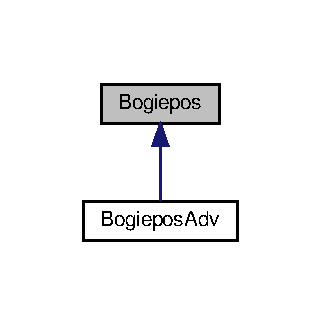
\includegraphics[width=154pt]{classBogiepos__inherit__graph}
\end{center}
\end{figure}


Collaboration diagram for Bogiepos\+:\nopagebreak
\begin{figure}[H]
\begin{center}
\leavevmode
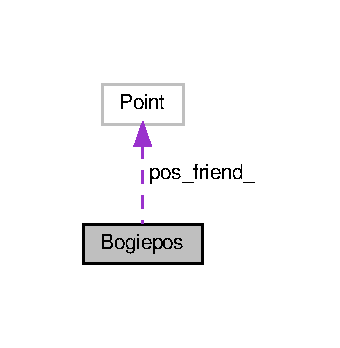
\includegraphics[width=163pt]{classBogiepos__coll__graph}
\end{center}
\end{figure}
\subsection*{Public Member Functions}
\begin{DoxyCompactItemize}
\item 
\hyperlink{classBogiepos_ad5db58b0f0ad66be505851ea9514d579}{Bogiepos} ()
\begin{DoxyCompactList}\small\item\em Construct a new \hyperlink{classBogiepos}{Bogiepos} object. \end{DoxyCompactList}\item 
\hyperlink{classBogiepos_a658f927c4ae34b41c7bd08b6a448b9cb}{Bogiepos} (std\+::shared\+\_\+ptr$<$ Simulator $>$ \&sim)
\begin{DoxyCompactList}\small\item\em Construct a new \hyperlink{classBogiepos}{Bogiepos} object. \end{DoxyCompactList}\item 
\mbox{\Hypertarget{classBogiepos_a6b1a0d5c052e6d4af5d1f55cd815ef7c}\label{classBogiepos_a6b1a0d5c052e6d4af5d1f55cd815ef7c}} 
\hyperlink{classBogiepos_a6b1a0d5c052e6d4af5d1f55cd815ef7c}{$\sim$\+Bogiepos} ()
\begin{DoxyCompactList}\small\item\em Destroy the \hyperlink{classBogiepos}{Bogiepos} object. \end{DoxyCompactList}\item 
\mbox{\Hypertarget{classBogiepos_a25b918db7e3b9b403d202216ddba636b}\label{classBogiepos_a25b918db7e3b9b403d202216ddba636b}} 
virtual void \hyperlink{classBogiepos_a25b918db7e3b9b403d202216ddba636b}{start} ()
\begin{DoxyCompactList}\small\item\em starts threads \end{DoxyCompactList}\item 
std\+::vector$<$ std\+::pair$<$ Point, double $>$ $>$ \hyperlink{classBogiepos_a513a373b97583009e8f6c2e487ba5b3a}{getbogiefriendly} ()
\begin{DoxyCompactList}\small\item\em Returns bogie positions in x,y from friendly frame of reference. Where the Point holds the x and y coords, z as range and the double is the angle to the bogie. \end{DoxyCompactList}\item 
std\+::vector$<$ std\+::pair$<$ Point, double $>$ $>$ \hyperlink{classBogiepos_abf7b5d2b2d099e51bfb46b1aaf8c797e}{getbogieglobal} ()
\begin{DoxyCompactList}\small\item\em Returns bogie positions in global frame of reference as a vector of points. \end{DoxyCompactList}\item 
std\+::pair$<$ Point, double $>$ \hyperlink{classBogiepos_a8bdb83f90cf5381b9c620a7fbc12a2dc}{getfriendlyxy0} ()
\begin{DoxyCompactList}\small\item\em Gets the friendly orientation. \end{DoxyCompactList}\item 
\mbox{\Hypertarget{classBogiepos_af5bf0a9ddc9540dcf8243f2041251949}\label{classBogiepos_af5bf0a9ddc9540dcf8243f2041251949}} 
std\+::map$<$ int, Point $>$ {\bfseries getmap} ()
\item 
Point \hyperlink{classBogiepos_a91b69776c48fd215112e60e7f6cc55fa}{global2local} (Point friendxy, double friendtheta, Point bogiepos)
\begin{DoxyCompactList}\small\item\em Calculates local bogie xy based on global coordinates. \end{DoxyCompactList}\item 
std\+::vector$<$ std\+::pair$<$ int, int $>$ $>$ \hyperlink{classBogiepos_af1bd0da948d84ba0a294adbc10bcbdca}{rangebearassociate} (std\+::vector$<$ Range\+Bearing\+Stamped $>$ rbs, Point friendxy)
\begin{DoxyCompactList}\small\item\em After an original call to rangebearingtobogiefrom\+Friendly and collected a set of 4 readings, a call to this function will relate a secondary set of readings from a second rangebearingtobogiefrom\+Frienly to the original. \end{DoxyCompactList}\item 
std\+::vector$<$ std\+::pair$<$ int, int $>$ $>$ \hyperlink{classBogiepos_aaaee6b3fa6631cb2893fe1824c2320e3}{rangevelassociate} (std\+::vector$<$ Range\+Velocity\+Stamped $>$ rvs)
\begin{DoxyCompactList}\small\item\em Same as above, except with readings from the base stations. \end{DoxyCompactList}\end{DoxyCompactItemize}
\subsection*{Protected Member Functions}
\begin{DoxyCompactItemize}
\item 
\mbox{\Hypertarget{classBogiepos_a4c8eedde0ce7c33ea7fe8e97aa6d412b}\label{classBogiepos_a4c8eedde0ce7c33ea7fe8e97aa6d412b}} 
void \hyperlink{classBogiepos_a4c8eedde0ce7c33ea7fe8e97aa6d412b}{getfriendinfo} ()
\begin{DoxyCompactList}\small\item\em Synchronises obtaining friendly info from sim using mutex. \end{DoxyCompactList}\item 
\mbox{\Hypertarget{classBogiepos_a35efba7b6086dcdd62f1ff60cd392ccd}\label{classBogiepos_a35efba7b6086dcdd62f1ff60cd392ccd}} 
void \hyperlink{classBogiepos_a35efba7b6086dcdd62f1ff60cd392ccd}{calcbogieglobalandfriendly} ()
\begin{DoxyCompactList}\small\item\em Top level thread that calls other functions above to calculate both bogies x,y in global and local frames of reference. \end{DoxyCompactList}\item 
std\+::pair$<$ Point, double $>$ \hyperlink{classBogiepos_a92af33e7edbae36591d1a564d9add2cc}{calcglobalxy} (Point rngbr, Point pos\+\_\+frnd, double theta)
\begin{DoxyCompactList}\small\item\em Calculates the global x and y based off local frame of reference and location. \end{DoxyCompactList}\item 
Point \hyperlink{classBogiepos_a48fc24fe51edd4e9835a141e369d5bd4}{calcfrndxy} (std\+::pair$<$ double, double $>$ rngbr)
\begin{DoxyCompactList}\small\item\em Calculates the x,y of bogie from friendly frame of reference. \end{DoxyCompactList}\item 
std\+::vector$<$ double $>$ \hyperlink{classBogiepos_a349025535b13e08322a94409e57873e9}{gettimes} ()
\begin{DoxyCompactList}\small\item\em Gets the timestaps of a given set of readings. Used in derived class bogiepos\+Adv to get the times for a set of rangebearing readings for the use of calculating bogie velocity. \end{DoxyCompactList}\end{DoxyCompactItemize}
\subsection*{Protected Attributes}
\begin{DoxyCompactItemize}
\item 
\mbox{\Hypertarget{classBogiepos_a34000659627785c6540cb80859feb581}\label{classBogiepos_a34000659627785c6540cb80859feb581}} 
std\+::atomic$<$ bool $>$ {\bfseries globalbogiesgot\+\_\+}
\item 
\mbox{\Hypertarget{classBogiepos_a078da1e8c36879c4a7814f1871a0cda2}\label{classBogiepos_a078da1e8c36879c4a7814f1871a0cda2}} 
std\+::atomic$<$ bool $>$ \hyperlink{classBogiepos_a078da1e8c36879c4a7814f1871a0cda2}{friendbogiesgot\+\_\+}
\begin{DoxyCompactList}\small\item\em boolean used for G\+Bcv\+\_\+ predicate. Triggered when global bogie xy has been calculated \end{DoxyCompactList}\item 
\mbox{\Hypertarget{classBogiepos_a738345d6726997c8a7500ed98a9071d8}\label{classBogiepos_a738345d6726997c8a7500ed98a9071d8}} 
std\+::atomic$<$ bool $>$ \hyperlink{classBogiepos_a738345d6726997c8a7500ed98a9071d8}{gottimes\+\_\+}
\begin{DoxyCompactList}\small\item\em boolean used for F\+Bcv\+\_\+ predicate. Triggered when local bogie xy has been calculated \end{DoxyCompactList}\item 
\mbox{\Hypertarget{classBogiepos_ad4e826244556b74fb218b183a932cbf8}\label{classBogiepos_ad4e826244556b74fb218b183a932cbf8}} 
std\+::atomic$<$ bool $>$ \hyperlink{classBogiepos_ad4e826244556b74fb218b183a932cbf8}{flying}
\begin{DoxyCompactList}\small\item\em boolean used for Tmcv\+\_\+ predicate. Triggered when timestamps have been collected \end{DoxyCompactList}\item 
\mbox{\Hypertarget{classBogiepos_a41790cca77f5ae39cc10978f48faf22f}\label{classBogiepos_a41790cca77f5ae39cc10978f48faf22f}} 
std\+::shared\+\_\+ptr$<$ Simulator $>$ \hyperlink{classBogiepos_a41790cca77f5ae39cc10978f48faf22f}{sim\+\_\+}
\begin{DoxyCompactList}\small\item\em boolean used to keep threads running \end{DoxyCompactList}\item 
\mbox{\Hypertarget{classBogiepos_acdafe3f586665301295284508f343d23}\label{classBogiepos_acdafe3f586665301295284508f343d23}} 
std\+::vector$<$ std\+::pair$<$ Point, double $>$ $>$ \hyperlink{classBogiepos_acdafe3f586665301295284508f343d23}{frnd\+\_\+bogies\+\_\+pos\+\_\+}
\begin{DoxyCompactList}\small\item\em class variable of simulator object. Shared between this class and \hyperlink{classControl}{Control} class \end{DoxyCompactList}\item 
\mbox{\Hypertarget{classBogiepos_aa642cf929d826b3ed1ae9fadb27323d6}\label{classBogiepos_aa642cf929d826b3ed1ae9fadb27323d6}} 
std\+::vector$<$ std\+::pair$<$ Point, double $>$ $>$ \hyperlink{classBogiepos_aa642cf929d826b3ed1ae9fadb27323d6}{glb\+\_\+bogies\+\_\+pos\+\_\+}
\begin{DoxyCompactList}\small\item\em vector containing bogie xy from friendly \end{DoxyCompactList}\item 
\mbox{\Hypertarget{classBogiepos_aa7750ca662f485c6374eb4bd074bdf00}\label{classBogiepos_aa7750ca662f485c6374eb4bd074bdf00}} 
std\+::vector$<$ double $>$ \hyperlink{classBogiepos_aa7750ca662f485c6374eb4bd074bdf00}{times\+\_\+}
\begin{DoxyCompactList}\small\item\em vector containint bogie xy in global coord \end{DoxyCompactList}\item 
\mbox{\Hypertarget{classBogiepos_ae6ca05a0ddb131bf0b66a5e35ceb30e4}\label{classBogiepos_ae6ca05a0ddb131bf0b66a5e35ceb30e4}} 
std\+::map$<$ int, Point $>$ {\bfseries m\+\_\+}
\item 
\mbox{\Hypertarget{classBogiepos_a8820b715858b2c25ebd45c7641da96a2}\label{classBogiepos_a8820b715858b2c25ebd45c7641da96a2}} 
std\+::vector$<$ Range\+Bearing\+Stamped $>$ \hyperlink{classBogiepos_a8820b715858b2c25ebd45c7641da96a2}{rbf\+\_\+}
\begin{DoxyCompactList}\small\item\em map which stores the index from an original set of 4 bogies to their global coords. Used in association \end{DoxyCompactList}\item 
\mbox{\Hypertarget{classBogiepos_a162e3d9be75bf8c0281ddbc56b40fb62}\label{classBogiepos_a162e3d9be75bf8c0281ddbc56b40fb62}} 
Point {\bfseries pos\+\_\+friend\+\_\+}
\item 
\mbox{\Hypertarget{classBogiepos_af473d776c1ed9edf9f1d8af85cd9ac35}\label{classBogiepos_af473d776c1ed9edf9f1d8af85cd9ac35}} 
double {\bfseries friend\+\_\+theta\+\_\+}
\item 
\mbox{\Hypertarget{classBogiepos_afb4793bea74a5b442242b16ccb58adef}\label{classBogiepos_afb4793bea74a5b442242b16ccb58adef}} 
std\+::vector$<$ std\+::thread $>$ {\bfseries threads\+\_\+}
\item 
\mbox{\Hypertarget{classBogiepos_aa4832d973bd9e51a759625d729a096c1}\label{classBogiepos_aa4832d973bd9e51a759625d729a096c1}} 
std\+::condition\+\_\+variable {\bfseries F\+Bcv\+\_\+}
\item 
\mbox{\Hypertarget{classBogiepos_a3c8228b9a0707d799b954f522c5e31ba}\label{classBogiepos_a3c8228b9a0707d799b954f522c5e31ba}} 
std\+::condition\+\_\+variable \hyperlink{classBogiepos_a3c8228b9a0707d799b954f522c5e31ba}{G\+Bcv\+\_\+}
\begin{DoxyCompactList}\small\item\em convar used to wait for bogie coords from friendly vector \end{DoxyCompactList}\item 
\mbox{\Hypertarget{classBogiepos_ac0860e78ea88ffa0ac9d52166c59136e}\label{classBogiepos_ac0860e78ea88ffa0ac9d52166c59136e}} 
std\+::condition\+\_\+variable \hyperlink{classBogiepos_ac0860e78ea88ffa0ac9d52166c59136e}{Tmcv\+\_\+}
\begin{DoxyCompactList}\small\item\em convar used to wait for bogie coords in global vector \end{DoxyCompactList}\item 
\mbox{\Hypertarget{classBogiepos_abfabc136eb8055dd32de540f6049c866}\label{classBogiepos_abfabc136eb8055dd32de540f6049c866}} 
std\+::mutex {\bfseries mtx\+\_\+}
\item 
\mbox{\Hypertarget{classBogiepos_a2726af1b3d3733b562e02e0a8693c5c3}\label{classBogiepos_a2726af1b3d3733b562e02e0a8693c5c3}} 
std\+::mutex \hyperlink{classBogiepos_a2726af1b3d3733b562e02e0a8693c5c3}{mtx2\+\_\+}
\begin{DoxyCompactList}\small\item\em mutex for glb\+\_\+bogie\+\_\+pos\+\_\+ \end{DoxyCompactList}\item 
\mbox{\Hypertarget{classBogiepos_a002263aed53cb021c2a296b06f92a4f4}\label{classBogiepos_a002263aed53cb021c2a296b06f92a4f4}} 
std\+::mutex \hyperlink{classBogiepos_a002263aed53cb021c2a296b06f92a4f4}{timemtx\+\_\+}
\begin{DoxyCompactList}\small\item\em mutex for frnd\+\_\+bogies\+\_\+pos\+\_\+ \end{DoxyCompactList}\item 
\mbox{\Hypertarget{classBogiepos_afb0fe54a6c6801619e2ae3560c5be15d}\label{classBogiepos_afb0fe54a6c6801619e2ae3560c5be15d}} 
bool {\bfseries basic}
\end{DoxyCompactItemize}


\subsection{Constructor \& Destructor Documentation}
\mbox{\Hypertarget{classBogiepos_ad5db58b0f0ad66be505851ea9514d579}\label{classBogiepos_ad5db58b0f0ad66be505851ea9514d579}} 
\index{Bogiepos@{Bogiepos}!Bogiepos@{Bogiepos}}
\index{Bogiepos@{Bogiepos}!Bogiepos@{Bogiepos}}
\subsubsection{\texorpdfstring{Bogiepos()}{Bogiepos()}\hspace{0.1cm}{\footnotesize\ttfamily [1/2]}}
{\footnotesize\ttfamily Bogiepos\+::\+Bogiepos (\begin{DoxyParamCaption}{ }\end{DoxyParamCaption})}



Construct a new \hyperlink{classBogiepos}{Bogiepos} object. 

\begin{DoxyNote}{Note}
Default constructor 
\end{DoxyNote}
\mbox{\Hypertarget{classBogiepos_a658f927c4ae34b41c7bd08b6a448b9cb}\label{classBogiepos_a658f927c4ae34b41c7bd08b6a448b9cb}} 
\index{Bogiepos@{Bogiepos}!Bogiepos@{Bogiepos}}
\index{Bogiepos@{Bogiepos}!Bogiepos@{Bogiepos}}
\subsubsection{\texorpdfstring{Bogiepos()}{Bogiepos()}\hspace{0.1cm}{\footnotesize\ttfamily [2/2]}}
{\footnotesize\ttfamily Bogiepos\+::\+Bogiepos (\begin{DoxyParamCaption}\item[{std\+::shared\+\_\+ptr$<$ Simulator $>$ \&}]{sim }\end{DoxyParamCaption})}



Construct a new \hyperlink{classBogiepos}{Bogiepos} object. 

\begin{DoxyNote}{Note}
The primary constructor that is called for use with the sim.
\end{DoxyNote}

\begin{DoxyParams}{Parameters}
{\em sim} & \\
\hline
\end{DoxyParams}


\subsection{Member Function Documentation}
\mbox{\Hypertarget{classBogiepos_a48fc24fe51edd4e9835a141e369d5bd4}\label{classBogiepos_a48fc24fe51edd4e9835a141e369d5bd4}} 
\index{Bogiepos@{Bogiepos}!calcfrndxy@{calcfrndxy}}
\index{calcfrndxy@{calcfrndxy}!Bogiepos@{Bogiepos}}
\subsubsection{\texorpdfstring{calcfrndxy()}{calcfrndxy()}}
{\footnotesize\ttfamily Point Bogiepos\+::calcfrndxy (\begin{DoxyParamCaption}\item[{std\+::pair$<$ double, double $>$}]{rngbr }\end{DoxyParamCaption})\hspace{0.3cm}{\ttfamily [protected]}}



Calculates the x,y of bogie from friendly frame of reference. 


\begin{DoxyParams}{Parameters}
{\em rngbr} & Pair holding range/bearing from sim function \\
\hline
\end{DoxyParams}
\begin{DoxyReturn}{Returns}
Point 
\end{DoxyReturn}
\mbox{\Hypertarget{classBogiepos_a92af33e7edbae36591d1a564d9add2cc}\label{classBogiepos_a92af33e7edbae36591d1a564d9add2cc}} 
\index{Bogiepos@{Bogiepos}!calcglobalxy@{calcglobalxy}}
\index{calcglobalxy@{calcglobalxy}!Bogiepos@{Bogiepos}}
\subsubsection{\texorpdfstring{calcglobalxy()}{calcglobalxy()}}
{\footnotesize\ttfamily std\+::pair$<$ Point, double $>$ Bogiepos\+::calcglobalxy (\begin{DoxyParamCaption}\item[{Point}]{rngbr,  }\item[{Point}]{pos\+\_\+frnd,  }\item[{double}]{theta }\end{DoxyParamCaption})\hspace{0.3cm}{\ttfamily [protected]}}



Calculates the global x and y based off local frame of reference and location. 


\begin{DoxyParams}{Parameters}
{\em rngbr} & Pair holding the range/bearing from sim function \\
\hline
{\em pos\+\_\+frnd} & position of friendly in global x,y \\
\hline
{\em theta} & orientation of friendly in global frame \\
\hline
\end{DoxyParams}
\begin{DoxyReturn}{Returns}
std\+::pair$<$\+Point,double$>$ 
\end{DoxyReturn}
\mbox{\Hypertarget{classBogiepos_a513a373b97583009e8f6c2e487ba5b3a}\label{classBogiepos_a513a373b97583009e8f6c2e487ba5b3a}} 
\index{Bogiepos@{Bogiepos}!getbogiefriendly@{getbogiefriendly}}
\index{getbogiefriendly@{getbogiefriendly}!Bogiepos@{Bogiepos}}
\subsubsection{\texorpdfstring{getbogiefriendly()}{getbogiefriendly()}}
{\footnotesize\ttfamily std\+::vector$<$ std\+::pair$<$ Point, double $>$ $>$ Bogiepos\+::getbogiefriendly (\begin{DoxyParamCaption}{ }\end{DoxyParamCaption})}



Returns bogie positions in x,y from friendly frame of reference. Where the Point holds the x and y coords, z as range and the double is the angle to the bogie. 

\begin{DoxyReturn}{Returns}
std\+::vector$<$std\+::pair$<$\+Point,double$>$$>$ 
\end{DoxyReturn}
\mbox{\Hypertarget{classBogiepos_abf7b5d2b2d099e51bfb46b1aaf8c797e}\label{classBogiepos_abf7b5d2b2d099e51bfb46b1aaf8c797e}} 
\index{Bogiepos@{Bogiepos}!getbogieglobal@{getbogieglobal}}
\index{getbogieglobal@{getbogieglobal}!Bogiepos@{Bogiepos}}
\subsubsection{\texorpdfstring{getbogieglobal()}{getbogieglobal()}}
{\footnotesize\ttfamily std\+::vector$<$ std\+::pair$<$ Point, double $>$ $>$ Bogiepos\+::getbogieglobal (\begin{DoxyParamCaption}{ }\end{DoxyParamCaption})}



Returns bogie positions in global frame of reference as a vector of points. 

\begin{DoxyReturn}{Returns}
std\+::vector$<$\+Point$>$ 
\end{DoxyReturn}
\mbox{\Hypertarget{classBogiepos_a8bdb83f90cf5381b9c620a7fbc12a2dc}\label{classBogiepos_a8bdb83f90cf5381b9c620a7fbc12a2dc}} 
\index{Bogiepos@{Bogiepos}!getfriendlyxy0@{getfriendlyxy0}}
\index{getfriendlyxy0@{getfriendlyxy0}!Bogiepos@{Bogiepos}}
\subsubsection{\texorpdfstring{getfriendlyxy0()}{getfriendlyxy0()}}
{\footnotesize\ttfamily std\+::pair$<$ Point, double $>$ Bogiepos\+::getfriendlyxy0 (\begin{DoxyParamCaption}{ }\end{DoxyParamCaption})}



Gets the friendly orientation. 

\begin{DoxyReturn}{Returns}
std\+::pair$<$\+Point,double$>$ 
\end{DoxyReturn}
\mbox{\Hypertarget{classBogiepos_a349025535b13e08322a94409e57873e9}\label{classBogiepos_a349025535b13e08322a94409e57873e9}} 
\index{Bogiepos@{Bogiepos}!gettimes@{gettimes}}
\index{gettimes@{gettimes}!Bogiepos@{Bogiepos}}
\subsubsection{\texorpdfstring{gettimes()}{gettimes()}}
{\footnotesize\ttfamily std\+::vector$<$ double $>$ Bogiepos\+::gettimes (\begin{DoxyParamCaption}{ }\end{DoxyParamCaption})\hspace{0.3cm}{\ttfamily [protected]}}



Gets the timestaps of a given set of readings. Used in derived class bogiepos\+Adv to get the times for a set of rangebearing readings for the use of calculating bogie velocity. 

\begin{DoxyReturn}{Returns}
std\+::vector$<$double$>$ 
\end{DoxyReturn}
\mbox{\Hypertarget{classBogiepos_a91b69776c48fd215112e60e7f6cc55fa}\label{classBogiepos_a91b69776c48fd215112e60e7f6cc55fa}} 
\index{Bogiepos@{Bogiepos}!global2local@{global2local}}
\index{global2local@{global2local}!Bogiepos@{Bogiepos}}
\subsubsection{\texorpdfstring{global2local()}{global2local()}}
{\footnotesize\ttfamily Point Bogiepos\+::global2local (\begin{DoxyParamCaption}\item[{Point}]{friendxy,  }\item[{double}]{friendtheta,  }\item[{Point}]{bogiepos }\end{DoxyParamCaption})}



Calculates local bogie xy based on global coordinates. 


\begin{DoxyParams}{Parameters}
{\em friendxy} & \\
\hline
{\em friendtheta} & \\
\hline
{\em bogiepos} & \\
\hline
\end{DoxyParams}
\begin{DoxyReturn}{Returns}
Point 
\end{DoxyReturn}
\mbox{\Hypertarget{classBogiepos_af1bd0da948d84ba0a294adbc10bcbdca}\label{classBogiepos_af1bd0da948d84ba0a294adbc10bcbdca}} 
\index{Bogiepos@{Bogiepos}!rangebearassociate@{rangebearassociate}}
\index{rangebearassociate@{rangebearassociate}!Bogiepos@{Bogiepos}}
\subsubsection{\texorpdfstring{rangebearassociate()}{rangebearassociate()}}
{\footnotesize\ttfamily std\+::vector$<$ std\+::pair$<$ int, int $>$ $>$ Bogiepos\+::rangebearassociate (\begin{DoxyParamCaption}\item[{std\+::vector$<$ Range\+Bearing\+Stamped $>$}]{rbs,  }\item[{Point}]{friendxy }\end{DoxyParamCaption})}



After an original call to rangebearingtobogiefrom\+Friendly and collected a set of 4 readings, a call to this function will relate a secondary set of readings from a second rangebearingtobogiefrom\+Frienly to the original. 


\begin{DoxyParams}{Parameters}
{\em rbs} & \\
\hline
{\em friendxy} & \\
\hline
\end{DoxyParams}
\begin{DoxyReturn}{Returns}
std\+::vector$<$std\+::pair$<$int,int$>$$>$ 
\end{DoxyReturn}
\mbox{\Hypertarget{classBogiepos_aaaee6b3fa6631cb2893fe1824c2320e3}\label{classBogiepos_aaaee6b3fa6631cb2893fe1824c2320e3}} 
\index{Bogiepos@{Bogiepos}!rangevelassociate@{rangevelassociate}}
\index{rangevelassociate@{rangevelassociate}!Bogiepos@{Bogiepos}}
\subsubsection{\texorpdfstring{rangevelassociate()}{rangevelassociate()}}
{\footnotesize\ttfamily std\+::vector$<$ std\+::pair$<$ int, int $>$ $>$ Bogiepos\+::rangevelassociate (\begin{DoxyParamCaption}\item[{std\+::vector$<$ Range\+Velocity\+Stamped $>$}]{rvs }\end{DoxyParamCaption})}



Same as above, except with readings from the base stations. 


\begin{DoxyParams}{Parameters}
{\em rvs} & \\
\hline
\end{DoxyParams}
\begin{DoxyReturn}{Returns}
std\+::vector$<$std\+::pair$<$int,int$>$$>$ 
\end{DoxyReturn}


The documentation for this class was generated from the following files\+:\begin{DoxyCompactItemize}
\item 
bogiepos.\+h\item 
bogiepos.\+cpp\end{DoxyCompactItemize}

\hypertarget{classBogieposAdv}{}\section{Bogiepos\+Adv Class Reference}
\label{classBogieposAdv}\index{Bogiepos\+Adv@{Bogiepos\+Adv}}


Inheritance diagram for Bogiepos\+Adv\+:\nopagebreak
\begin{figure}[H]
\begin{center}
\leavevmode
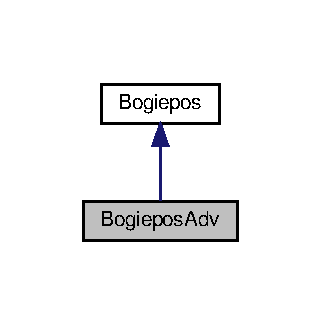
\includegraphics[width=154pt]{classBogieposAdv__inherit__graph}
\end{center}
\end{figure}


Collaboration diagram for Bogiepos\+Adv\+:\nopagebreak
\begin{figure}[H]
\begin{center}
\leavevmode
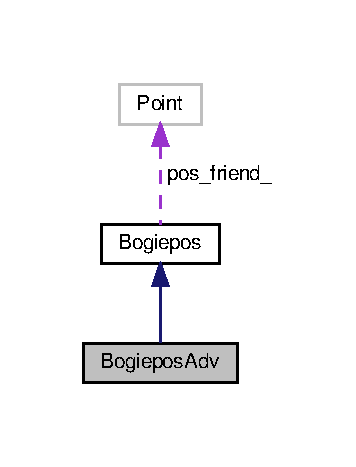
\includegraphics[width=171pt]{classBogieposAdv__coll__graph}
\end{center}
\end{figure}
\subsection*{Public Member Functions}
\begin{DoxyCompactItemize}
\item 
\mbox{\Hypertarget{classBogieposAdv_a0b295babf5011077561b9bb8729f9ac2}\label{classBogieposAdv_a0b295babf5011077561b9bb8729f9ac2}} 
{\bfseries Bogiepos\+Adv} (std\+::shared\+\_\+ptr$<$ Simulator $>$ \&sim, std\+::shared\+\_\+ptr$<$ Timer $>$ \&timer)
\item 
\mbox{\Hypertarget{classBogieposAdv_a0d2aa854b7d981dcd2aab317c6647004}\label{classBogieposAdv_a0d2aa854b7d981dcd2aab317c6647004}} 
void \hyperlink{classBogieposAdv_a0d2aa854b7d981dcd2aab317c6647004}{start} ()
\begin{DoxyCompactList}\small\item\em starts threads \end{DoxyCompactList}\item 
\mbox{\Hypertarget{classBogieposAdv_a56ebed2f7f60d2983c16154a966ed9e3}\label{classBogieposAdv_a56ebed2f7f60d2983c16154a966ed9e3}} 
std\+::map$<$ int, \hyperlink{structvelocity}{velocity} $>$ {\bfseries calcbogie\+Vel} ()
\item 
\mbox{\Hypertarget{classBogieposAdv_a4854019d616648248d766bf014c56ff7}\label{classBogieposAdv_a4854019d616648248d766bf014c56ff7}} 
\hyperlink{structvelocity}{velocity} {\bfseries getvel} (std\+::pair$<$ int, int $>$ \&it, std\+::vector$<$ std\+::pair$<$ Point, double $>$$>$ \&t1, std\+::vector$<$ std\+::pair$<$ Point, double $>$$>$ \&t0, std\+::vector$<$ double $>$ \&times1, std\+::vector$<$ double $>$ \&times0, double \&pose)
\end{DoxyCompactItemize}
\subsection*{Protected Member Functions}
\begin{DoxyCompactItemize}
\item 
\mbox{\Hypertarget{classBogieposAdv_a1397ca8153862494414ff135997da59a}\label{classBogieposAdv_a1397ca8153862494414ff135997da59a}} 
std\+::vector$<$ std\+::pair$<$ int, int $>$ $>$ {\bfseries associate} (std\+::vector$<$ std\+::pair$<$ Point, double $>$$>$ \&vec1, std\+::vector$<$ std\+::pair$<$ Point, double $>$$>$ \&vec2)
\end{DoxyCompactItemize}
\subsection*{Protected Attributes}
\begin{DoxyCompactItemize}
\item 
\mbox{\Hypertarget{classBogieposAdv_a4fd97d2f8f9ba65028cc3f92960ce2db}\label{classBogieposAdv_a4fd97d2f8f9ba65028cc3f92960ce2db}} 
std\+::shared\+\_\+ptr$<$ Timer $>$ {\bfseries timer\+\_\+}
\item 
\mbox{\Hypertarget{classBogieposAdv_aaba3fb9369708bc8b21c10aab41d7441}\label{classBogieposAdv_aaba3fb9369708bc8b21c10aab41d7441}} 
std\+::map$<$ int, \hyperlink{structvelocity}{velocity} $>$ {\bfseries bogie\+\_\+ids}
\item 
\mbox{\Hypertarget{classBogieposAdv_ab23f42b77901d0a6add7364a3a63b77c}\label{classBogieposAdv_ab23f42b77901d0a6add7364a3a63b77c}} 
std\+::condition\+\_\+variable {\bfseries Velcv\+\_\+}
\item 
\mbox{\Hypertarget{classBogieposAdv_adfe1922b518765c4f6ca3f496597d81f}\label{classBogieposAdv_adfe1922b518765c4f6ca3f496597d81f}} 
std\+::mutex {\bfseries Velmtx\+\_\+}
\item 
\mbox{\Hypertarget{classBogieposAdv_a6cd66259846f16c3025c3bb0cb06239a}\label{classBogieposAdv_a6cd66259846f16c3025c3bb0cb06239a}} 
bool {\bfseries getvelocities\+\_\+}
\end{DoxyCompactItemize}


The documentation for this class was generated from the following files\+:\begin{DoxyCompactItemize}
\item 
bogiepos\+Adv.\+h\item 
bogiepos\+Adv.\+cpp\end{DoxyCompactItemize}

\hypertarget{classBogieposInterface}{}\section{Bogiepos\+Interface Class Reference}
\label{classBogieposInterface}\index{Bogiepos\+Interface@{Bogiepos\+Interface}}


Bogpieposition Interface Class.  




{\ttfamily \#include $<$bogieposinterface.\+h$>$}



Collaboration diagram for Bogiepos\+Interface\+:\nopagebreak
\begin{figure}[H]
\begin{center}
\leavevmode
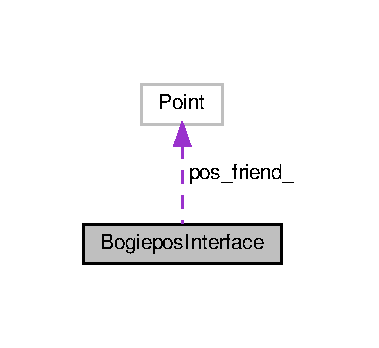
\includegraphics[width=182pt]{classBogieposInterface__coll__graph}
\end{center}
\end{figure}
\subsection*{Public Member Functions}
\begin{DoxyCompactItemize}
\item 
\mbox{\Hypertarget{classBogieposInterface_a2a1a87b14e16f622d5acb694c9b9fcc0}\label{classBogieposInterface_a2a1a87b14e16f622d5acb694c9b9fcc0}} 
virtual void \hyperlink{classBogieposInterface_a2a1a87b14e16f622d5acb694c9b9fcc0}{start} ()=0
\begin{DoxyCompactList}\small\item\em starts threads \end{DoxyCompactList}\item 
std\+::vector$<$ std\+::pair$<$ Point, double $>$ $>$ \hyperlink{classBogieposInterface_aed3b03940731c8235e29795bdc493bbd}{getbogiefriendly} ()
\begin{DoxyCompactList}\small\item\em Returns bogie positions in x,y from friendly frame of reference. Where the Point holds the x and y coords, z as range and the double is the angle to the bogie. \end{DoxyCompactList}\item 
std\+::vector$<$ std\+::pair$<$ Point, double $>$ $>$ \hyperlink{classBogieposInterface_a0b8ba02bf6deb7b647f075e838bbbca9}{getbogieglobal} ()
\begin{DoxyCompactList}\small\item\em Returns bogie positions in global frame of reference as a vector of points. \end{DoxyCompactList}\item 
std\+::pair$<$ Point, double $>$ \hyperlink{classBogieposInterface_a730cb8dcbd3c42a19b6f6350ec1e3999}{getfriendlyxy0} ()
\begin{DoxyCompactList}\small\item\em Gets the friendly orientation. \end{DoxyCompactList}\item 
\mbox{\Hypertarget{classBogieposInterface_af3e26b24f89b107056e086ed0bc5e1c1}\label{classBogieposInterface_af3e26b24f89b107056e086ed0bc5e1c1}} 
void \hyperlink{classBogieposInterface_af3e26b24f89b107056e086ed0bc5e1c1}{getfriendinfo} ()
\begin{DoxyCompactList}\small\item\em Synchronises obtaining friendly info from sim using mutex. \end{DoxyCompactList}\item 
\mbox{\Hypertarget{classBogieposInterface_a4cdda06dbe106fa960365d9f59ba572f}\label{classBogieposInterface_a4cdda06dbe106fa960365d9f59ba572f}} 
void \hyperlink{classBogieposInterface_a4cdda06dbe106fa960365d9f59ba572f}{calcbogieglobalandfriendly} ()
\begin{DoxyCompactList}\small\item\em Top level thread that calls other functions above to calculate both bogies x,y in global and local frames of reference. \end{DoxyCompactList}\item 
std\+::pair$<$ Point, double $>$ \hyperlink{classBogieposInterface_a0d6962250b64da519be1e8ac46a7afa7}{calcglobalxy} (Point rngbr, Point pos\+\_\+frnd, double theta)
\begin{DoxyCompactList}\small\item\em Calculates the global x and y based off local frame of reference and location. \end{DoxyCompactList}\item 
Point \hyperlink{classBogieposInterface_abdbf2caf087cb39dcf35700ecf9128bd}{calcfrndxy} (std\+::pair$<$ double, double $>$ rngbr)
\begin{DoxyCompactList}\small\item\em Calculates the x,y of bogie from friendly frame of reference. \end{DoxyCompactList}\end{DoxyCompactItemize}
\subsection*{Public Attributes}
\begin{DoxyCompactItemize}
\item 
\mbox{\Hypertarget{classBogieposInterface_a5e1fd43a4b2bf930fc62e933282bec19}\label{classBogieposInterface_a5e1fd43a4b2bf930fc62e933282bec19}} 
std\+::atomic$<$ bool $>$ {\bfseries globalbogiesgot\+\_\+}
\item 
\mbox{\Hypertarget{classBogieposInterface_a861afcebc5fb09e17f2e3b32922c9678}\label{classBogieposInterface_a861afcebc5fb09e17f2e3b32922c9678}} 
std\+::atomic$<$ bool $>$ \hyperlink{classBogieposInterface_a861afcebc5fb09e17f2e3b32922c9678}{friendbogiesgot\+\_\+}
\begin{DoxyCompactList}\small\item\em test \end{DoxyCompactList}\item 
\mbox{\Hypertarget{classBogieposInterface_a5caf6590a0e805f00fcfd472d48130ed}\label{classBogieposInterface_a5caf6590a0e805f00fcfd472d48130ed}} 
std\+::atomic$<$ bool $>$ {\bfseries flying}
\item 
\mbox{\Hypertarget{classBogieposInterface_a408d1de1da6941e99911a9af9f9875e2}\label{classBogieposInterface_a408d1de1da6941e99911a9af9f9875e2}} 
std\+::atomic$<$ bool $>$ {\bfseries friendly\+\_\+info}
\item 
\mbox{\Hypertarget{classBogieposInterface_a80006e18bc4928eccc493937c891ce7c}\label{classBogieposInterface_a80006e18bc4928eccc493937c891ce7c}} 
std\+::shared\+\_\+ptr$<$ Simulator $>$ {\bfseries sim\+\_\+}
\item 
\mbox{\Hypertarget{classBogieposInterface_a1ce4e6797926bb18ef24c6bdd7372093}\label{classBogieposInterface_a1ce4e6797926bb18ef24c6bdd7372093}} 
std\+::vector$<$ std\+::pair$<$ Point, double $>$ $>$ {\bfseries frnd\+\_\+bogies\+\_\+pos\+\_\+}
\item 
\mbox{\Hypertarget{classBogieposInterface_a3d4d80384d8372890c53068ccac2f734}\label{classBogieposInterface_a3d4d80384d8372890c53068ccac2f734}} 
std\+::vector$<$ std\+::pair$<$ Point, double $>$ $>$ {\bfseries glb\+\_\+bogies\+\_\+pos\+\_\+}
\item 
\mbox{\Hypertarget{classBogieposInterface_a3a77385b1c98cf6047dd8c5ba880b19a}\label{classBogieposInterface_a3a77385b1c98cf6047dd8c5ba880b19a}} 
std\+::vector$<$ Range\+Bearing\+Stamped $>$ {\bfseries rbf\+\_\+}
\item 
\mbox{\Hypertarget{classBogieposInterface_a033c04b5ccf5753d998d429ca3d9e557}\label{classBogieposInterface_a033c04b5ccf5753d998d429ca3d9e557}} 
Point {\bfseries pos\+\_\+friend\+\_\+}
\item 
\mbox{\Hypertarget{classBogieposInterface_a8e8826e05c8ac240093b2278e241579f}\label{classBogieposInterface_a8e8826e05c8ac240093b2278e241579f}} 
double {\bfseries friend\+\_\+theta\+\_\+}
\item 
\mbox{\Hypertarget{classBogieposInterface_afeb37637f67ddeb44bfa8916c512e5d5}\label{classBogieposInterface_afeb37637f67ddeb44bfa8916c512e5d5}} 
std\+::vector$<$ std\+::thread $>$ {\bfseries threads\+\_\+}
\item 
\mbox{\Hypertarget{classBogieposInterface_a91170e4a4f7b4b1b5ce8af5070e48162}\label{classBogieposInterface_a91170e4a4f7b4b1b5ce8af5070e48162}} 
std\+::condition\+\_\+variable {\bfseries cv\+\_\+}
\item 
\mbox{\Hypertarget{classBogieposInterface_a721c81d1b0c28dd1849b311654bcc427}\label{classBogieposInterface_a721c81d1b0c28dd1849b311654bcc427}} 
std\+::condition\+\_\+variable {\bfseries F\+Bcv\+\_\+}
\item 
\mbox{\Hypertarget{classBogieposInterface_afd6361c4d8c896f52eddfffaca18df6b}\label{classBogieposInterface_afd6361c4d8c896f52eddfffaca18df6b}} 
std\+::condition\+\_\+variable {\bfseries G\+Bcv\+\_\+}
\item 
\mbox{\Hypertarget{classBogieposInterface_a01943e42e9d6279885f51de115158db9}\label{classBogieposInterface_a01943e42e9d6279885f51de115158db9}} 
std\+::mutex {\bfseries mtx\+\_\+}
\item 
\mbox{\Hypertarget{classBogieposInterface_a013edcb6bc5eb8b238b307fe71594230}\label{classBogieposInterface_a013edcb6bc5eb8b238b307fe71594230}} 
std\+::mutex {\bfseries mtx2\+\_\+}
\end{DoxyCompactItemize}


\subsection{Detailed Description}
Bogpieposition Interface Class. 

This interface class is used to set all the methods that need to be embodies within any subsequent derived sensor classes. \begin{DoxyAuthor}{Author}
Joseph Seklawy 
\end{DoxyAuthor}
\begin{DoxyVersion}{Version}
1.\+0 
\end{DoxyVersion}
\begin{DoxyDate}{Date}
2021-\/10-\/07 
\end{DoxyDate}


\subsection{Member Function Documentation}
\mbox{\Hypertarget{classBogieposInterface_abdbf2caf087cb39dcf35700ecf9128bd}\label{classBogieposInterface_abdbf2caf087cb39dcf35700ecf9128bd}} 
\index{Bogiepos\+Interface@{Bogiepos\+Interface}!calcfrndxy@{calcfrndxy}}
\index{calcfrndxy@{calcfrndxy}!Bogiepos\+Interface@{Bogiepos\+Interface}}
\subsubsection{\texorpdfstring{calcfrndxy()}{calcfrndxy()}}
{\footnotesize\ttfamily Point Bogiepos\+Interface\+::calcfrndxy (\begin{DoxyParamCaption}\item[{std\+::pair$<$ double, double $>$}]{rngbr }\end{DoxyParamCaption})}



Calculates the x,y of bogie from friendly frame of reference. 


\begin{DoxyParams}{Parameters}
{\em rngbr} & Pair holding range/bearing from sim function \\
\hline
\end{DoxyParams}
\begin{DoxyReturn}{Returns}
Point 
\end{DoxyReturn}
\mbox{\Hypertarget{classBogieposInterface_a0d6962250b64da519be1e8ac46a7afa7}\label{classBogieposInterface_a0d6962250b64da519be1e8ac46a7afa7}} 
\index{Bogiepos\+Interface@{Bogiepos\+Interface}!calcglobalxy@{calcglobalxy}}
\index{calcglobalxy@{calcglobalxy}!Bogiepos\+Interface@{Bogiepos\+Interface}}
\subsubsection{\texorpdfstring{calcglobalxy()}{calcglobalxy()}}
{\footnotesize\ttfamily std\+::pair$<$Point,double$>$ Bogiepos\+Interface\+::calcglobalxy (\begin{DoxyParamCaption}\item[{Point}]{rngbr,  }\item[{Point}]{pos\+\_\+frnd,  }\item[{double}]{theta }\end{DoxyParamCaption})}



Calculates the global x and y based off local frame of reference and location. 


\begin{DoxyParams}{Parameters}
{\em rngbr} & Pair holding the range/bearing from sim function \\
\hline
{\em pos\+\_\+frnd} & position of friendly in global x,y \\
\hline
{\em theta} & orientation of friendly in global frame \\
\hline
\end{DoxyParams}
\begin{DoxyReturn}{Returns}
std\+::pair$<$\+Point,double$>$ 
\end{DoxyReturn}
\mbox{\Hypertarget{classBogieposInterface_aed3b03940731c8235e29795bdc493bbd}\label{classBogieposInterface_aed3b03940731c8235e29795bdc493bbd}} 
\index{Bogiepos\+Interface@{Bogiepos\+Interface}!getbogiefriendly@{getbogiefriendly}}
\index{getbogiefriendly@{getbogiefriendly}!Bogiepos\+Interface@{Bogiepos\+Interface}}
\subsubsection{\texorpdfstring{getbogiefriendly()}{getbogiefriendly()}}
{\footnotesize\ttfamily std\+::vector$<$std\+::pair$<$Point,double$>$ $>$ Bogiepos\+Interface\+::getbogiefriendly (\begin{DoxyParamCaption}{ }\end{DoxyParamCaption})}



Returns bogie positions in x,y from friendly frame of reference. Where the Point holds the x and y coords, z as range and the double is the angle to the bogie. 

\begin{DoxyReturn}{Returns}
std\+::vector$<$std\+::pair$<$\+Point,double$>$$>$ 
\end{DoxyReturn}
\mbox{\Hypertarget{classBogieposInterface_a0b8ba02bf6deb7b647f075e838bbbca9}\label{classBogieposInterface_a0b8ba02bf6deb7b647f075e838bbbca9}} 
\index{Bogiepos\+Interface@{Bogiepos\+Interface}!getbogieglobal@{getbogieglobal}}
\index{getbogieglobal@{getbogieglobal}!Bogiepos\+Interface@{Bogiepos\+Interface}}
\subsubsection{\texorpdfstring{getbogieglobal()}{getbogieglobal()}}
{\footnotesize\ttfamily std\+::vector$<$std\+::pair$<$Point,double$>$ $>$ Bogiepos\+Interface\+::getbogieglobal (\begin{DoxyParamCaption}{ }\end{DoxyParamCaption})}



Returns bogie positions in global frame of reference as a vector of points. 

\begin{DoxyReturn}{Returns}
std\+::vector$<$\+Point$>$ 
\end{DoxyReturn}
\mbox{\Hypertarget{classBogieposInterface_a730cb8dcbd3c42a19b6f6350ec1e3999}\label{classBogieposInterface_a730cb8dcbd3c42a19b6f6350ec1e3999}} 
\index{Bogiepos\+Interface@{Bogiepos\+Interface}!getfriendlyxy0@{getfriendlyxy0}}
\index{getfriendlyxy0@{getfriendlyxy0}!Bogiepos\+Interface@{Bogiepos\+Interface}}
\subsubsection{\texorpdfstring{getfriendlyxy0()}{getfriendlyxy0()}}
{\footnotesize\ttfamily std\+::pair$<$Point,double$>$ Bogiepos\+Interface\+::getfriendlyxy0 (\begin{DoxyParamCaption}{ }\end{DoxyParamCaption})}



Gets the friendly orientation. 

\begin{DoxyReturn}{Returns}
std\+::pair$<$\+Point,double$>$ 
\end{DoxyReturn}


The documentation for this class was generated from the following file\+:\begin{DoxyCompactItemize}
\item 
bogieposinterface.\+h\end{DoxyCompactItemize}

\hypertarget{classControl}{}\section{Control Class Reference}
\label{classControl}\index{Control@{Control}}


Inheritance diagram for Control\+:\nopagebreak
\begin{figure}[H]
\begin{center}
\leavevmode
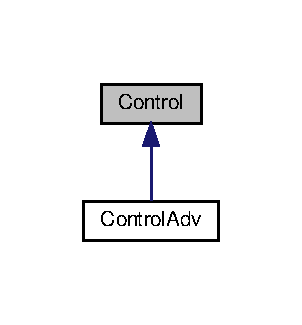
\includegraphics[width=145pt]{classControl__inherit__graph}
\end{center}
\end{figure}
\subsection*{Public Member Functions}
\begin{DoxyCompactItemize}
\item 
\mbox{\Hypertarget{classControl_a343774819922207def027e98b0bc3198}\label{classControl_a343774819922207def027e98b0bc3198}} 
{\bfseries Control} (std\+::shared\+\_\+ptr$<$ Simulator $>$ \&sim)
\item 
\mbox{\Hypertarget{classControl_a933994a3524f2f6d7ef0a17086e7cf66}\label{classControl_a933994a3524f2f6d7ef0a17086e7cf66}} 
virtual void \hyperlink{classControl_a933994a3524f2f6d7ef0a17086e7cf66}{start} ()
\begin{DoxyCompactList}\small\item\em starts threads \end{DoxyCompactList}\item 
bool \hyperlink{classControl_af7401b14ae40f38234d29b6adaf5d8a6}{getrestart} ()
\begin{DoxyCompactList}\small\item\em Public getter called in main once 4 bogies have been intercepted to allow for new readings to be recieved. \end{DoxyCompactList}\item 
virtual void \hyperlink{classControl_aff1c1cb4117bcdff659978feb6d45a8f}{setbogiexyth} (std\+::vector$<$ std\+::pair$<$ Point, double $>$$>$ \&bogiexyth, std\+::vector$<$ std\+::pair$<$ Point, double $>$$>$ \&bogieglb, std\+::pair$<$ Point, double $>$ frnd, std\+::map$<$ int, Point $>$ map)
\begin{DoxyCompactList}\small\item\em Called in the main to take data from \hyperlink{classBogiepos}{Bogiepos} class into object of this class. \end{DoxyCompactList}\end{DoxyCompactItemize}
\subsection*{Protected Member Functions}
\begin{DoxyCompactItemize}
\item 
\mbox{\Hypertarget{classControl_a11fd8f10f43a8375262c0b1cc34d73ff}\label{classControl_a11fd8f10f43a8375262c0b1cc34d73ff}} 
void {\bfseries move} ()
\item 
\mbox{\Hypertarget{classControl_a4e088c3e3a959fa80b2055a615ee946e}\label{classControl_a4e088c3e3a959fa80b2055a615ee946e}} 
void \hyperlink{classControl_a4e088c3e3a959fa80b2055a615ee946e}{idle} ()
\begin{DoxyCompactList}\small\item\em Ensures watchdog timer is satisfied. \end{DoxyCompactList}\item 
void \hyperlink{classControl_aa18094ca515f8dbcdff94e0b7a60a88a}{command} (double lin, double ang)
\begin{DoxyCompactList}\small\item\em issues velocity commands \end{DoxyCompactList}\item 
void \hyperlink{classControl_a9bfe498567206c176b0e23d71708d6e3}{calcpath} ()
\begin{DoxyCompactList}\small\item\em Main thread calculates bogie order via graph search. \end{DoxyCompactList}\item 
void \hyperlink{classControl_af846dd07501030d430893f17cd4a4178}{getoptimalpath} (std\+::vector$<$ int $>$ \&optpath)
\begin{DoxyCompactList}\small\item\em function inside \hyperlink{classControl_a9bfe498567206c176b0e23d71708d6e3}{calcpath()} \end{DoxyCompactList}\item 
double \hyperlink{classControl_a57ae0e13099f01e27fe5afc0765bc611}{wrapalpha} (double alpha)
\begin{DoxyCompactList}\small\item\em wraps angle between 0-\/\+PI or -\/\+P\+I-\/0 \end{DoxyCompactList}\item 
double \hyperlink{classControl_a3535c9d84af21822fe3b5318391092b1}{relate\+Orientto\+B\+Bangle} (double orient, double bearing)
\begin{DoxyCompactList}\small\item\em Relates the bearing angle of a bogie from base to the needed friendly orientation to be pointed at the bogie. \end{DoxyCompactList}\item 
int \hyperlink{classControl_a3b1ef3f00ba7fdee871d352d7d5f546e}{graphsearch} (int node, double \&quickest\+\_\+time, double \&current\+\_\+orient)
\begin{DoxyCompactList}\small\item\em Graph search function called in optpath. \end{DoxyCompactList}\item 
\mbox{\Hypertarget{classControl_a1282c47a9b0a0b6b9d5c19dd4cfa2764}\label{classControl_a1282c47a9b0a0b6b9d5c19dd4cfa2764}} 
virtual void \hyperlink{classControl_a1282c47a9b0a0b6b9d5c19dd4cfa2764}{optvelocities} ()
\begin{DoxyCompactList}\small\item\em Calculates the needed linear and angular velocites to achieve the pure pursuit gamma function. \end{DoxyCompactList}\item 
\mbox{\Hypertarget{classControl_abdb51463e49b88bde90c97c2c72d3148}\label{classControl_abdb51463e49b88bde90c97c2c72d3148}} 
std\+::vector$<$ std\+::pair$<$ int, int $>$ $>$ {\bfseries rangebearassociate} (std\+::vector$<$ Range\+Bearing\+Stamped $>$ rbs, Point friendxy)
\end{DoxyCompactItemize}
\subsection*{Protected Attributes}
\begin{DoxyCompactItemize}
\item 
\mbox{\Hypertarget{classControl_a603378c110983f3c855df10bfe525c8e}\label{classControl_a603378c110983f3c855df10bfe525c8e}} 
std\+::mutex {\bfseries mtxpos\+\_\+}
\item 
\mbox{\Hypertarget{classControl_aab035f20a9ed6ef18761e9fad3403b79}\label{classControl_aab035f20a9ed6ef18761e9fad3403b79}} 
std\+::mutex \hyperlink{classControl_aab035f20a9ed6ef18761e9fad3403b79}{Cmdmtx\+\_\+}
\begin{DoxyCompactList}\small\item\em mutex for cv\+\_\+ convar \end{DoxyCompactList}\item 
\mbox{\Hypertarget{classControl_a2e77b6aaf947cb52490bb0ae6fbbc404}\label{classControl_a2e77b6aaf947cb52490bb0ae6fbbc404}} 
std\+::mutex \hyperlink{classControl_a2e77b6aaf947cb52490bb0ae6fbbc404}{Velmtx\+\_\+}
\begin{DoxyCompactList}\small\item\em command mutex, used for sending move commands via lin\+\_\+vel\+\_\+ and ang\+\_\+vel\+\_\+ \end{DoxyCompactList}\item 
\mbox{\Hypertarget{classControl_aec807365dbda609b3d3df8f8e9a3b565}\label{classControl_aec807365dbda609b3d3df8f8e9a3b565}} 
std\+::condition\+\_\+variable {\bfseries cv\+\_\+}
\item 
\mbox{\Hypertarget{classControl_aa8fb0e7eb4a78e85d07cecb3c95d47f9}\label{classControl_aa8fb0e7eb4a78e85d07cecb3c95d47f9}} 
std\+::condition\+\_\+variable \hyperlink{classControl_aa8fb0e7eb4a78e85d07cecb3c95d47f9}{Movecv\+\_\+}
\begin{DoxyCompactList}\small\item\em convar used to wake up main \hyperlink{classControl_a9bfe498567206c176b0e23d71708d6e3}{calcpath()} thread once bogie xy has been collected from bogiepos object \end{DoxyCompactList}\item 
\mbox{\Hypertarget{classControl_a786552cb46cde87e5d8aac8da769df8f}\label{classControl_a786552cb46cde87e5d8aac8da769df8f}} 
std\+::condition\+\_\+variable {\bfseries Velcv\+\_\+}
\item 
\mbox{\Hypertarget{classControl_afe4abd7bbf2c1a1d21ffa037ddf8ee82}\label{classControl_afe4abd7bbf2c1a1d21ffa037ddf8ee82}} 
std\+::vector$<$ std\+::thread $>$ \hyperlink{classControl_afe4abd7bbf2c1a1d21ffa037ddf8ee82}{threads\+\_\+}
\begin{DoxyCompactList}\small\item\em convar used to wake up function which supplied sim with velocities which moves friendly towards bogies \end{DoxyCompactList}\item 
\mbox{\Hypertarget{classControl_a2183b81bba807e732f8cd768e99c6e20}\label{classControl_a2183b81bba807e732f8cd768e99c6e20}} 
std\+::atomic$<$ bool $>$ {\bfseries running\+\_\+}
\item 
\mbox{\Hypertarget{classControl_a77748ccf7bb58ffa0b280ad7e33a2f9e}\label{classControl_a77748ccf7bb58ffa0b280ad7e33a2f9e}} 
std\+::atomic$<$ bool $>$ \hyperlink{classControl_a77748ccf7bb58ffa0b280ad7e33a2f9e}{gotbogies\+\_\+}
\begin{DoxyCompactList}\small\item\em bool to keep threads running when true \end{DoxyCompactList}\item 
\mbox{\Hypertarget{classControl_adf8a05b46c15032b9d7cc72f9b2b5d6e}\label{classControl_adf8a05b46c15032b9d7cc72f9b2b5d6e}} 
std\+::atomic$<$ bool $>$ \hyperlink{classControl_adf8a05b46c15032b9d7cc72f9b2b5d6e}{gotpath\+\_\+}
\begin{DoxyCompactList}\small\item\em boolean used for cv\+\_\+ predicate. Set to true when data from bogiepos class has come through \end{DoxyCompactList}\item 
\mbox{\Hypertarget{classControl_afde9de0840660562bfb1d4adaf513a58}\label{classControl_afde9de0840660562bfb1d4adaf513a58}} 
std\+::atomic$<$ bool $>$ \hyperlink{classControl_afde9de0840660562bfb1d4adaf513a58}{gotglobal\+\_\+}
\begin{DoxyCompactList}\small\item\em boolean used to notify when a bogie order has been determined \end{DoxyCompactList}\item 
\mbox{\Hypertarget{classControl_ac976ca5679155e87d0d48439515385f6}\label{classControl_ac976ca5679155e87d0d48439515385f6}} 
std\+::atomic$<$ bool $>$ {\bfseries getvel\+\_\+}
\item 
\mbox{\Hypertarget{classControl_a7eda266577684041424f5f30b83e7c61}\label{classControl_a7eda266577684041424f5f30b83e7c61}} 
std\+::atomic$<$ bool $>$ \hyperlink{classControl_a7eda266577684041424f5f30b83e7c61}{startmove\+\_\+}
\begin{DoxyCompactList}\small\item\em boolean set to true once pure pursuit gamma has been calculated. Allows for combination of angular and linear velocity to be calculated to match gamma \end{DoxyCompactList}\item 
\mbox{\Hypertarget{classControl_acbae7d5fe1e846d3e18bde050b7d47eb}\label{classControl_acbae7d5fe1e846d3e18bde050b7d47eb}} 
std\+::shared\+\_\+ptr$<$ Simulator $>$ \hyperlink{classControl_acbae7d5fe1e846d3e18bde050b7d47eb}{sim\+\_\+}
\begin{DoxyCompactList}\small\item\em once velocity from above has been calculated set to true to begin moving \end{DoxyCompactList}\item 
\mbox{\Hypertarget{classControl_af8f3f9e1cdc0eef72c8909fb4fdbe625}\label{classControl_af8f3f9e1cdc0eef72c8909fb4fdbe625}} 
bool {\bfseries restart\+\_\+}
\item 
\mbox{\Hypertarget{classControl_a1f1ff7bfd8ae9d904b0129a7aa5d9423}\label{classControl_a1f1ff7bfd8ae9d904b0129a7aa5d9423}} 
std\+::vector$<$ std\+::pair$<$ Point, double $>$ $>$ {\bfseries bogiexyth\+\_\+}
\item 
\mbox{\Hypertarget{classControl_a619045e6557f64b899094072d91cb81c}\label{classControl_a619045e6557f64b899094072d91cb81c}} 
std\+::vector$<$ std\+::pair$<$ Point, double $>$ $>$ {\bfseries bogieglb\+\_\+}
\item 
\mbox{\Hypertarget{classControl_ab08189ab85b36a617ca92fe0d5c883f9}\label{classControl_ab08189ab85b36a617ca92fe0d5c883f9}} 
double {\bfseries friend\+\_\+orient}
\item 
\mbox{\Hypertarget{classControl_ae0c72e0e6f9a65c47e465919d933f591}\label{classControl_ae0c72e0e6f9a65c47e465919d933f591}} 
double {\bfseries lin\+\_\+vel\+\_\+}
\item 
\mbox{\Hypertarget{classControl_aad6d7018e96b5fa63eaa408efbe27a5d}\label{classControl_aad6d7018e96b5fa63eaa408efbe27a5d}} 
double {\bfseries ang\+\_\+vel\+\_\+}
\item 
\mbox{\Hypertarget{classControl_a24a6dc661cdf3860042fe413da5e0263}\label{classControl_a24a6dc661cdf3860042fe413da5e0263}} 
double {\bfseries gamma\+\_\+}
\item 
\mbox{\Hypertarget{classControl_a90725edeeaf742703b571edb950be39c}\label{classControl_a90725edeeaf742703b571edb950be39c}} 
bool {\bfseries base\+\_\+start}
\item 
\mbox{\Hypertarget{classControl_a3e85346d55044ad264e2806f4d50f75d}\label{classControl_a3e85346d55044ad264e2806f4d50f75d}} 
std\+::map$<$ int, Point $>$ {\bfseries map\+\_\+}
\item 
\mbox{\Hypertarget{classControl_a8b9b711bca4a1d3d796c4943141b2d46}\label{classControl_a8b9b711bca4a1d3d796c4943141b2d46}} 
std\+::vector$<$ std\+::pair$<$ Point, double $>$ $>$ {\bfseries P\+OI}
\item 
\mbox{\Hypertarget{classControl_a4f42fcf3ec3958ee4fd8cedfd34ed3c4}\label{classControl_a4f42fcf3ec3958ee4fd8cedfd34ed3c4}} 
std\+::vector$<$ std\+::pair$<$ double, double $>$ $>$ {\bfseries P\+O\+I\+\_\+sort\+\_\+}
\item 
\mbox{\Hypertarget{classControl_a306e59dd2abffd5dc259e49cd0d11250}\label{classControl_a306e59dd2abffd5dc259e49cd0d11250}} 
std\+::vector$<$ std\+::vector$<$ std\+::pair$<$ \hyperlink{structD__A}{D\+\_\+A}, int $>$ $>$ $>$ {\bfseries B\+Bgraph}
\item 
\mbox{\Hypertarget{classControl_a9fffc0076b66e557907e84e429c8e859}\label{classControl_a9fffc0076b66e557907e84e429c8e859}} 
std\+::vector$<$ int $>$ {\bfseries graph\+\_\+path}
\item 
\mbox{\Hypertarget{classControl_a9f281d802d134300f3583f5d14388eb9}\label{classControl_a9f281d802d134300f3583f5d14388eb9}} 
std\+::vector$<$ int $>$ {\bfseries opt\+\_\+path\+\_\+}
\end{DoxyCompactItemize}


\subsection{Member Function Documentation}
\mbox{\Hypertarget{classControl_a9bfe498567206c176b0e23d71708d6e3}\label{classControl_a9bfe498567206c176b0e23d71708d6e3}} 
\index{Control@{Control}!calcpath@{calcpath}}
\index{calcpath@{calcpath}!Control@{Control}}
\subsubsection{\texorpdfstring{calcpath()}{calcpath()}}
{\footnotesize\ttfamily void Control\+::calcpath (\begin{DoxyParamCaption}{ }\end{DoxyParamCaption})\hspace{0.3cm}{\ttfamily [protected]}}



Main thread calculates bogie order via graph search. 

Calculates time to each bogie from starting position //////////// \mbox{\Hypertarget{classControl_aa18094ca515f8dbcdff94e0b7a60a88a}\label{classControl_aa18094ca515f8dbcdff94e0b7a60a88a}} 
\index{Control@{Control}!command@{command}}
\index{command@{command}!Control@{Control}}
\subsubsection{\texorpdfstring{command()}{command()}}
{\footnotesize\ttfamily void Control\+::command (\begin{DoxyParamCaption}\item[{double}]{lin,  }\item[{double}]{ang }\end{DoxyParamCaption})\hspace{0.3cm}{\ttfamily [protected]}}



issues velocity commands 


\begin{DoxyParams}{Parameters}
{\em lin} & \\
\hline
{\em ang} & \\
\hline
\end{DoxyParams}
\mbox{\Hypertarget{classControl_af846dd07501030d430893f17cd4a4178}\label{classControl_af846dd07501030d430893f17cd4a4178}} 
\index{Control@{Control}!getoptimalpath@{getoptimalpath}}
\index{getoptimalpath@{getoptimalpath}!Control@{Control}}
\subsubsection{\texorpdfstring{getoptimalpath()}{getoptimalpath()}}
{\footnotesize\ttfamily void Control\+::getoptimalpath (\begin{DoxyParamCaption}\item[{std\+::vector$<$ int $>$ \&}]{optpath }\end{DoxyParamCaption})\hspace{0.3cm}{\ttfamily [protected]}}



function inside \hyperlink{classControl_a9bfe498567206c176b0e23d71708d6e3}{calcpath()} 


\begin{DoxyParams}{Parameters}
{\em optpath} & \\
\hline
\end{DoxyParams}
\mbox{\Hypertarget{classControl_af7401b14ae40f38234d29b6adaf5d8a6}\label{classControl_af7401b14ae40f38234d29b6adaf5d8a6}} 
\index{Control@{Control}!getrestart@{getrestart}}
\index{getrestart@{getrestart}!Control@{Control}}
\subsubsection{\texorpdfstring{getrestart()}{getrestart()}}
{\footnotesize\ttfamily bool Control\+::getrestart (\begin{DoxyParamCaption}{ }\end{DoxyParamCaption})}



Public getter called in main once 4 bogies have been intercepted to allow for new readings to be recieved. 

\begin{DoxyReturn}{Returns}
true 

false 
\end{DoxyReturn}
\mbox{\Hypertarget{classControl_a3b1ef3f00ba7fdee871d352d7d5f546e}\label{classControl_a3b1ef3f00ba7fdee871d352d7d5f546e}} 
\index{Control@{Control}!graphsearch@{graphsearch}}
\index{graphsearch@{graphsearch}!Control@{Control}}
\subsubsection{\texorpdfstring{graphsearch()}{graphsearch()}}
{\footnotesize\ttfamily int Control\+::graphsearch (\begin{DoxyParamCaption}\item[{int}]{node,  }\item[{double \&}]{quickest\+\_\+time,  }\item[{double \&}]{current\+\_\+orient }\end{DoxyParamCaption})\hspace{0.3cm}{\ttfamily [protected]}}



Graph search function called in optpath. 


\begin{DoxyParams}{Parameters}
{\em node} & \\
\hline
{\em quickest\+\_\+time} & \\
\hline
{\em current\+\_\+orient} & \\
\hline
\end{DoxyParams}
\begin{DoxyReturn}{Returns}
int 
\end{DoxyReturn}
\mbox{\Hypertarget{classControl_a3535c9d84af21822fe3b5318391092b1}\label{classControl_a3535c9d84af21822fe3b5318391092b1}} 
\index{Control@{Control}!relate\+Orientto\+B\+Bangle@{relate\+Orientto\+B\+Bangle}}
\index{relate\+Orientto\+B\+Bangle@{relate\+Orientto\+B\+Bangle}!Control@{Control}}
\subsubsection{\texorpdfstring{relate\+Orientto\+B\+Bangle()}{relateOrienttoBBangle()}}
{\footnotesize\ttfamily double Control\+::relate\+Orientto\+B\+Bangle (\begin{DoxyParamCaption}\item[{double}]{orient,  }\item[{double}]{bearing }\end{DoxyParamCaption})\hspace{0.3cm}{\ttfamily [protected]}}



Relates the bearing angle of a bogie from base to the needed friendly orientation to be pointed at the bogie. 


\begin{DoxyParams}{Parameters}
{\em orient} & \\
\hline
{\em bearing} & \\
\hline
\end{DoxyParams}
\begin{DoxyReturn}{Returns}
double 
\end{DoxyReturn}
\mbox{\Hypertarget{classControl_aff1c1cb4117bcdff659978feb6d45a8f}\label{classControl_aff1c1cb4117bcdff659978feb6d45a8f}} 
\index{Control@{Control}!setbogiexyth@{setbogiexyth}}
\index{setbogiexyth@{setbogiexyth}!Control@{Control}}
\subsubsection{\texorpdfstring{setbogiexyth()}{setbogiexyth()}}
{\footnotesize\ttfamily void Control\+::setbogiexyth (\begin{DoxyParamCaption}\item[{std\+::vector$<$ std\+::pair$<$ Point, double $>$$>$ \&}]{bogiexyth,  }\item[{std\+::vector$<$ std\+::pair$<$ Point, double $>$$>$ \&}]{bogieglb,  }\item[{std\+::pair$<$ Point, double $>$}]{frnd,  }\item[{std\+::map$<$ int, Point $>$}]{map }\end{DoxyParamCaption})\hspace{0.3cm}{\ttfamily [virtual]}}



Called in the main to take data from \hyperlink{classBogiepos}{Bogiepos} class into object of this class. 


\begin{DoxyParams}{Parameters}
{\em bogiexyth} & \\
\hline
{\em bogieglb} & \\
\hline
{\em frnd} & \\
\hline
\end{DoxyParams}
\mbox{\Hypertarget{classControl_a57ae0e13099f01e27fe5afc0765bc611}\label{classControl_a57ae0e13099f01e27fe5afc0765bc611}} 
\index{Control@{Control}!wrapalpha@{wrapalpha}}
\index{wrapalpha@{wrapalpha}!Control@{Control}}
\subsubsection{\texorpdfstring{wrapalpha()}{wrapalpha()}}
{\footnotesize\ttfamily double Control\+::wrapalpha (\begin{DoxyParamCaption}\item[{double}]{alpha }\end{DoxyParamCaption})\hspace{0.3cm}{\ttfamily [protected]}}



wraps angle between 0-\/\+PI or -\/\+P\+I-\/0 


\begin{DoxyParams}{Parameters}
{\em alpha} & \\
\hline
\end{DoxyParams}
\begin{DoxyReturn}{Returns}
double 
\end{DoxyReturn}


The documentation for this class was generated from the following files\+:\begin{DoxyCompactItemize}
\item 
control.\+h\item 
control.\+cpp\end{DoxyCompactItemize}

\hypertarget{classControlAdv}{}\section{Control\+Adv Class Reference}
\label{classControlAdv}\index{Control\+Adv@{Control\+Adv}}


Inheritance diagram for Control\+Adv\+:\nopagebreak
\begin{figure}[H]
\begin{center}
\leavevmode
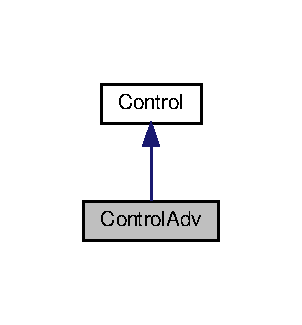
\includegraphics[width=145pt]{classControlAdv__inherit__graph}
\end{center}
\end{figure}


Collaboration diagram for Control\+Adv\+:\nopagebreak
\begin{figure}[H]
\begin{center}
\leavevmode
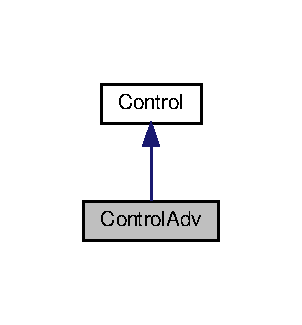
\includegraphics[width=145pt]{classControlAdv__coll__graph}
\end{center}
\end{figure}
\subsection*{Public Member Functions}
\begin{DoxyCompactItemize}
\item 
\mbox{\Hypertarget{classControlAdv_ac7548cd0591b7dfbac40b057a7eafa47}\label{classControlAdv_ac7548cd0591b7dfbac40b057a7eafa47}} 
{\bfseries Control\+Adv} (std\+::shared\+\_\+ptr$<$ Simulator $>$ \&sim, std\+::shared\+\_\+ptr$<$ Timer $>$ \&timer)
\item 
\mbox{\Hypertarget{classControlAdv_a6a7d6ff44d04141ace8bda9dc051dae0}\label{classControlAdv_a6a7d6ff44d04141ace8bda9dc051dae0}} 
void \hyperlink{classControlAdv_a6a7d6ff44d04141ace8bda9dc051dae0}{start} ()
\begin{DoxyCompactList}\small\item\em starts threads \end{DoxyCompactList}\item 
\mbox{\Hypertarget{classControlAdv_aca6b996dfb7b0633d0e402f0a09f7fdf}\label{classControlAdv_aca6b996dfb7b0633d0e402f0a09f7fdf}} 
void {\bfseries setbogiexyth} (std\+::map$<$ int, \hyperlink{structvelocity}{velocity} $>$ \&bogievel)
\item 
\mbox{\Hypertarget{classControlAdv_a069aae3738a7fb894acfcd49fb1fc129}\label{classControlAdv_a069aae3738a7fb894acfcd49fb1fc129}} 
void {\bfseries extrapbogiexy} (\hyperlink{structvelocity}{velocity} vel, double T, double \&ty, double \&tx)
\end{DoxyCompactItemize}
\subsection*{Private Member Functions}
\begin{DoxyCompactItemize}
\item 
\mbox{\Hypertarget{classControlAdv_af959e09368ce3cb3f514df163d56910b}\label{classControlAdv_af959e09368ce3cb3f514df163d56910b}} 
void {\bfseries calcintercept} ()
\item 
\mbox{\Hypertarget{classControlAdv_a9090a1f95722a0f8da3c6564b954c809}\label{classControlAdv_a9090a1f95722a0f8da3c6564b954c809}} 
double {\bfseries get\+Friendly\+Vx\+Vy} (double orient)
\item 
\mbox{\Hypertarget{classControlAdv_acd2da96b69355864cd786643934da6f4}\label{classControlAdv_acd2da96b69355864cd786643934da6f4}} 
void {\bfseries chase} ()
\item 
\mbox{\Hypertarget{classControlAdv_a488478a3a2b7cd2f36d5169ad6dd7781}\label{classControlAdv_a488478a3a2b7cd2f36d5169ad6dd7781}} 
void \hyperlink{classControlAdv_a488478a3a2b7cd2f36d5169ad6dd7781}{optvelocities} ()
\begin{DoxyCompactList}\small\item\em Calculates the needed linear and angular velocites to achieve the pure pursuit gamma function. \end{DoxyCompactList}\item 
\mbox{\Hypertarget{classControlAdv_a3264e85aeca962cfe7c635a320db865e}\label{classControlAdv_a3264e85aeca962cfe7c635a320db865e}} 
void {\bfseries idle} ()
\end{DoxyCompactItemize}
\subsection*{Private Attributes}
\begin{DoxyCompactItemize}
\item 
\mbox{\Hypertarget{classControlAdv_a086fbf6bfcadcf4d13d6116a5ce2e244}\label{classControlAdv_a086fbf6bfcadcf4d13d6116a5ce2e244}} 
std\+::condition\+\_\+variable {\bfseries velcv\+\_\+}
\item 
\mbox{\Hypertarget{classControlAdv_aea416263a252da236cc1a071f831a46e}\label{classControlAdv_aea416263a252da236cc1a071f831a46e}} 
std\+::mutex {\bfseries velmtx\+\_\+}
\item 
\mbox{\Hypertarget{classControlAdv_aab5412362f3266f03f65c47c43fb6f71}\label{classControlAdv_aab5412362f3266f03f65c47c43fb6f71}} 
std\+::shared\+\_\+ptr$<$ Timer $>$ {\bfseries timer\+\_\+}
\item 
\mbox{\Hypertarget{classControlAdv_ad42217b48fd54b942e742e659dbafeda}\label{classControlAdv_ad42217b48fd54b942e742e659dbafeda}} 
std\+::map$<$ int, \hyperlink{structvelocity}{velocity} $>$ {\bfseries bogie\+Vels\+\_\+}
\item 
\mbox{\Hypertarget{classControlAdv_a5e51c2094503e07e79a1e5908917ffd0}\label{classControlAdv_a5e51c2094503e07e79a1e5908917ffd0}} 
double {\bfseries velocity\+\_\+}
\item 
\mbox{\Hypertarget{classControlAdv_ad0f0eb876e33108e6ad8aec21b5a8339}\label{classControlAdv_ad0f0eb876e33108e6ad8aec21b5a8339}} 
double {\bfseries Vtheta\+\_\+}
\item 
\mbox{\Hypertarget{classControlAdv_a56e974bfba67286059caf386fe48fd73}\label{classControlAdv_a56e974bfba67286059caf386fe48fd73}} 
double {\bfseries b\+T\+\_\+theta\+\_\+}
\item 
\mbox{\Hypertarget{classControlAdv_a86a4c88f409e23090fec297853adaaa5}\label{classControlAdv_a86a4c88f409e23090fec297853adaaa5}} 
double {\bfseries bx\+T\+\_\+}
\item 
\mbox{\Hypertarget{classControlAdv_abcf06279afa676bf65c35d50c6521c15}\label{classControlAdv_abcf06279afa676bf65c35d50c6521c15}} 
double {\bfseries by\+T\+\_\+}
\item 
\mbox{\Hypertarget{classControlAdv_a3c7c48fe736574c6dcb360eb56371f44}\label{classControlAdv_a3c7c48fe736574c6dcb360eb56371f44}} 
std\+::atomic$<$ bool $>$ {\bfseries gotbogievels\+\_\+}
\end{DoxyCompactItemize}
\subsection*{Additional Inherited Members}


The documentation for this class was generated from the following files\+:\begin{DoxyCompactItemize}
\item 
control\+Adv.\+h\item 
control\+Adv.\+cpp\end{DoxyCompactItemize}

\hypertarget{structD__A}{}\section{D\+\_\+A Struct Reference}
\label{structD__A}\index{D\+\_\+A@{D\+\_\+A}}
\subsection*{Public Attributes}
\begin{DoxyCompactItemize}
\item 
\mbox{\Hypertarget{structD__A_a0adcbf6ddc78650737322a9f5cc1fa06}\label{structD__A_a0adcbf6ddc78650737322a9f5cc1fa06}} 
double {\bfseries dist}
\item 
\mbox{\Hypertarget{structD__A_a5dfb99bfdf59de1d782e725b1385dc52}\label{structD__A_a5dfb99bfdf59de1d782e725b1385dc52}} 
double {\bfseries angle}
\end{DoxyCompactItemize}


The documentation for this struct was generated from the following file\+:\begin{DoxyCompactItemize}
\item 
control.\+h\end{DoxyCompactItemize}

\hypertarget{structvelocity}{}\section{velocity Struct Reference}
\label{structvelocity}\index{velocity@{velocity}}
\subsection*{Public Attributes}
\begin{DoxyCompactItemize}
\item 
\mbox{\Hypertarget{structvelocity_af782cf3f02556d206dafb4fc215e8d56}\label{structvelocity_af782cf3f02556d206dafb4fc215e8d56}} 
double {\bfseries vx}
\item 
\mbox{\Hypertarget{structvelocity_a9c63e355e599ade6afb059290220ca68}\label{structvelocity_a9c63e355e599ade6afb059290220ca68}} 
double {\bfseries vy}
\item 
\mbox{\Hypertarget{structvelocity_a045bd9da67384da5b1a9a9338ee1581b}\label{structvelocity_a045bd9da67384da5b1a9a9338ee1581b}} 
double {\bfseries m}
\item 
\mbox{\Hypertarget{structvelocity_a93abe62f9c5fe1d96d72a04feb2bc64d}\label{structvelocity_a93abe62f9c5fe1d96d72a04feb2bc64d}} 
double {\bfseries x0}
\item 
\mbox{\Hypertarget{structvelocity_ace3302b327e857b708a315b05919e420}\label{structvelocity_ace3302b327e857b708a315b05919e420}} 
double {\bfseries y0}
\item 
\mbox{\Hypertarget{structvelocity_a47ca52e47c0a52f43d7888fb8743f824}\label{structvelocity_a47ca52e47c0a52f43d7888fb8743f824}} 
long {\bfseries time}
\end{DoxyCompactItemize}


The documentation for this struct was generated from the following file\+:\begin{DoxyCompactItemize}
\item 
bogiepos\+Adv.\+h\end{DoxyCompactItemize}

\hypertarget{structXY}{}\section{XY Struct Reference}
\label{structXY}\index{XY@{XY}}
\subsection*{Public Attributes}
\begin{DoxyCompactItemize}
\item 
\mbox{\Hypertarget{structXY_a4d12443240fd1aebc164deac323e5b96}\label{structXY_a4d12443240fd1aebc164deac323e5b96}} 
double {\bfseries x}
\item 
\mbox{\Hypertarget{structXY_a89d0178ba6dabee476d0576496c9b197}\label{structXY_a89d0178ba6dabee476d0576496c9b197}} 
double {\bfseries y}
\end{DoxyCompactItemize}


The documentation for this struct was generated from the following file\+:\begin{DoxyCompactItemize}
\item 
control.\+h\end{DoxyCompactItemize}

\chapter{File Documentation}
\hypertarget{main_8cpp}{}\section{main.\+cpp File Reference}
\label{main_8cpp}\index{main.\+cpp@{main.\+cpp}}


Main entry point for assignment 2.  


{\ttfamily \#include $<$thread$>$}\newline
{\ttfamily \#include $<$vector$>$}\newline
{\ttfamily \#include $<$iostream$>$}\newline
{\ttfamily \#include \char`\"{}dep/include/simulator.\+h\char`\"{}}\newline
{\ttfamily \#include \char`\"{}bogiepos.\+h\char`\"{}}\newline
{\ttfamily \#include \char`\"{}control.\+h\char`\"{}}\newline
{\ttfamily \#include \char`\"{}bogiepos\+Adv.\+h\char`\"{}}\newline
{\ttfamily \#include \char`\"{}control\+Adv.\+h\char`\"{}}\newline
Include dependency graph for main.\+cpp\+:\nopagebreak
\begin{figure}[H]
\begin{center}
\leavevmode
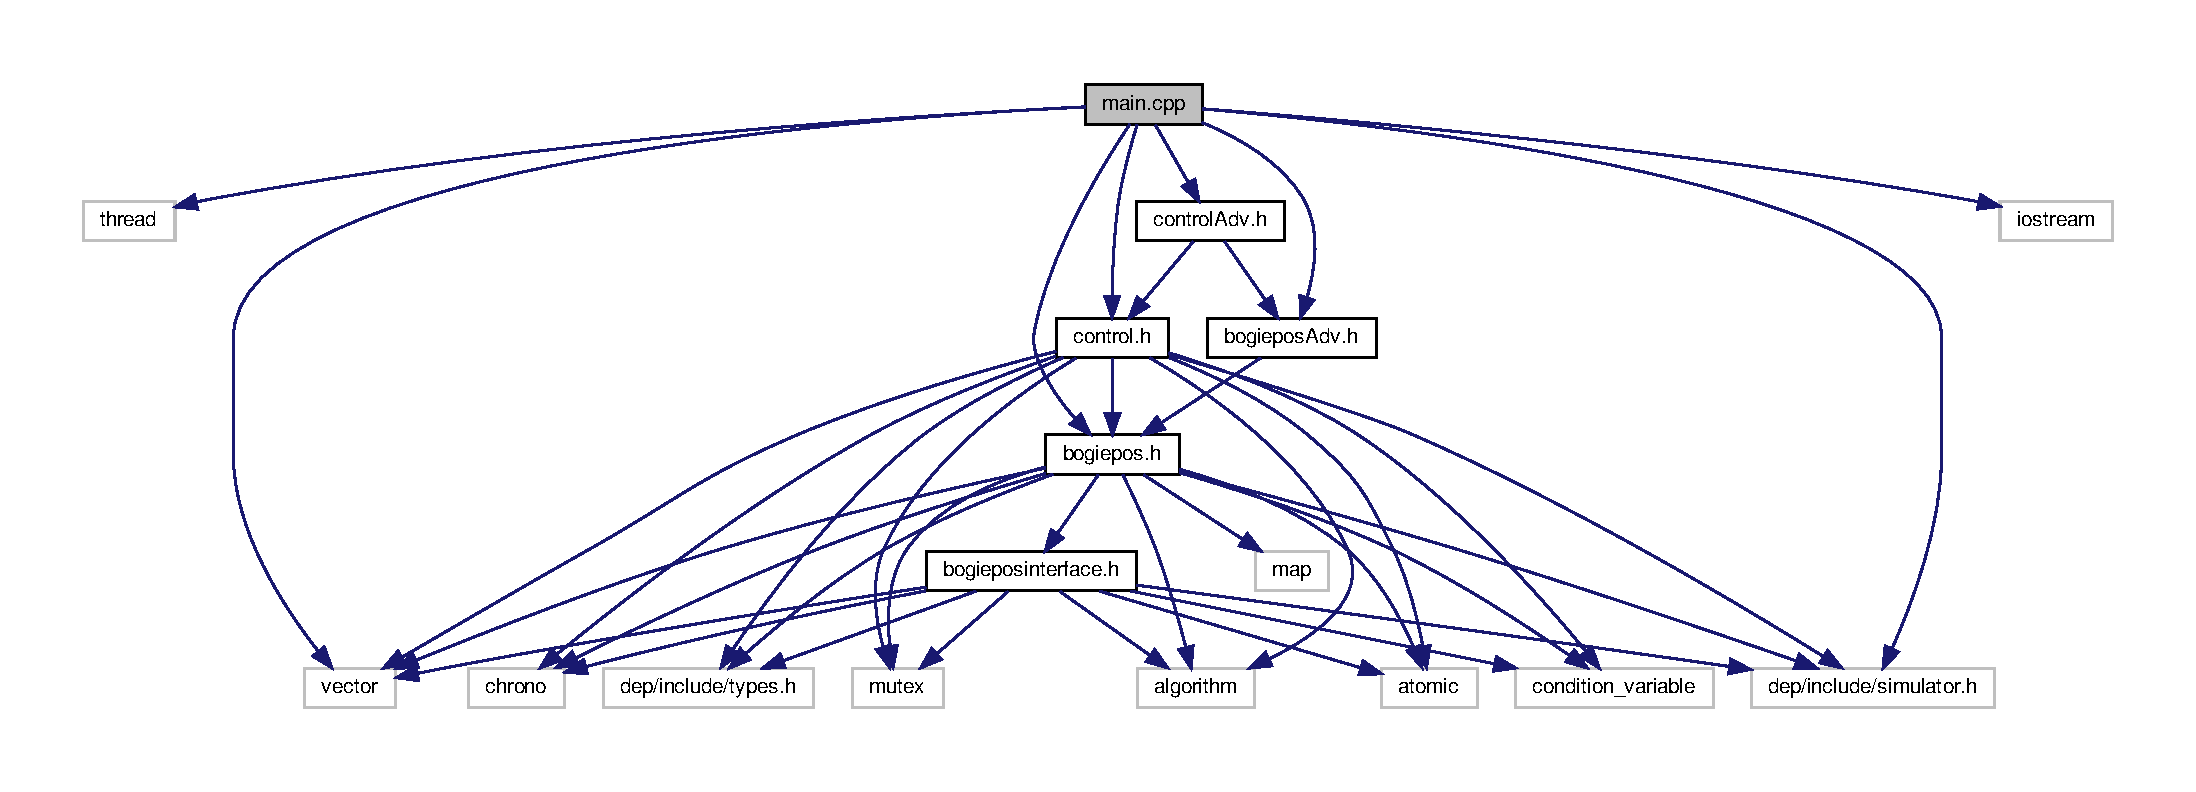
\includegraphics[width=350pt]{main_8cpp__incl}
\end{center}
\end{figure}
\subsection*{Functions}
\begin{DoxyCompactItemize}
\item 
\mbox{\Hypertarget{main_8cpp_a0ddf1224851353fc92bfbff6f499fa97}\label{main_8cpp_a0ddf1224851353fc92bfbff6f499fa97}} 
int {\bfseries main} (int argc, char $\ast$argv\mbox{[}$\,$\mbox{]})
\end{DoxyCompactItemize}


\subsection{Detailed Description}
Main entry point for assignment 2. 

T\+O\+DO\+: Add information here

\begin{DoxyAuthor}{Author}
Joseph Seklawy 12578845\{T\+O\+DO\+: Your student name + id\} 
\end{DoxyAuthor}
\begin{DoxyDate}{Date}
20/09/2021\{T\+O\+DO\} 
\end{DoxyDate}

%--- End generated contents ---

% Index
\backmatter
\newpage
\phantomsection
\clearemptydoublepage
\addcontentsline{toc}{chapter}{Index}
\printindex

\end{document}
